\documentclass[class=pmath370,tikz,notes]{agony}
\usetikzlibrary{external}
\tikzexternalize[prefix=figures-cache/]
\tikzset{external/only named=true}

\title{PMATH 370 Winter 2024: Lecture Notes}
\begin{document}
\renewcommand{\contentsname}{PMATH 370 Winter 2024:\\{\huge Lecture Notes}}
\thispagestyle{firstpage}
\tableofcontents

Lecture notes taken, unless otherwise specified,
by myself during the Winter 2024 offering of PMATH 370,
taught by Blake Madill.

\begin{multicols}{2}
  \listoflecture
\end{multicols}

\chapter{Iteration and Orbits}

\section{Orbits}
\lecture{Jan 8}

\begin{defn}[iteration]
  Let $f : A \to \R$ such that $A \subseteq \R$ and $f(A) \subseteq A$.
  For $a \in A$ we may \term[iteration]{iterate} the function at $a$:
  \[ x_1 = a, x_2 = f(a), x_3 = \underbrace{f(f(a))}_{f^2(a)}, \dotsc, x_i = f^{i-1}(a), \dotsc. \]
  The sequence $(x_n)_{n=1}^\infty$ is the \term[orbit]{orbit of $a$ under $f$}
  (abbreviated $(x_n)$ without limits).
\end{defn}

\begin{example}
  Let $f(x) = x^4 + 2x^2 - 2$, $a = -1$. What is the orbit of $a$ under $f$?
\end{example}
\begin{sol}
  $a = -1$, $f(a) = 1$, $f(f(a)) = f(1) = 1$, so we have $-1,1,1,1,\dotsc$.
  We call this eventually constant.
\end{sol}

\begin{example}
  Let $f(x) = -x^2 - x + 1$, $a = 0$. What is the orbit of $a$ under $f$?
\end{example}
\begin{sol}
  Calculate: $0, 1, -1, 1, -1, 1, \dotsc$.
  We call this eventually periodic (with period 2).
\end{sol}

\begin{example}
  Let $f(x) = x^3 - 3x + 1$, $a = 1$. What is the orbit of $a$ under $f$?
\end{example}
\begin{sol}
  Calculate the first few terms: $1, -1, 3, 19, \dotsc$ (too big).
  This is a divergence to infinity.
\end{sol}

\begin{example}
  Let $f(x) = x^2 + 2x$, $a = -0.5$. What is the orbit of $a$ under $f$?
\end{example}
\begin{sol}
  Calculate: $-0.5, -0.75, -0.9375, -0.9961\dots$
  and we make an educated guess that this converges to $-1$
  since $f(-1) = -1$, a fixed point.
\end{sol}

\begin{example}
  Let $f(x) = x^3 - 3x$, $a = 0.75$. What is the orbit of $a$ under $f$?
\end{example}
\begin{sol}
  Calculate: $0.75, -1.828, -0.625, 1.631, -0.552, \dotsc$.
  There is no clear pattern, so we call this chaotic.
  In fact, the orbit is dense in a neighbourhood of 0.
\end{sol}

We can start to formalize the examples.

\begin{defn}[fixed point]
  Let $f : A \to \R$ such that $f(A) \subseteq A$.
  A point $a \in A$ is fixed if $f(a) = a$.

  Then, the orbit of $a$ under $f$ is $(a,a,a,\dotsc)$
  which is \term[orbit!constant]{constant}.
\end{defn}

\begin{example}
  Find all fixed points of $f(x) = x^2 + x - 4$.
\end{example}
\begin{sol}
  We find points where $f(x) = x$, i.e., $x^2 + x - 4 = x$.
  \begin{equation*}
    x^2 + x - 4 = x \iff x^2 = 4 \iff x = \pm 2 \qedhere
  \end{equation*}
\end{sol}

\begin{example}\label{ex:graph}
  How many fixed points does $f(x) = 2\sin x$ have?
\end{example}
\begin{sol}
  Consider where the curve $y = 2\sin x$ meets $y = x$:
  \begin{center}
    \begin{tikzpicture}
      \begin{axis}[axis lines=middle,
          xlabel=$x$,
          ylabel=$y$,
          enlargelimits,
          ytick=\empty,
          xtick=\empty,
          samples=60]
        \addplot[name path=F,blue,domain={-6:6}] {2*sin(deg(x))} node[pos=.9, below]{$y = 2\sin x$};
        \addplot[name path=G,ForestGreen,domain={-4:4}] {x} node[pos=.8, left]{$y = x$};
      \end{axis}
    \end{tikzpicture}
  \end{center}
  We can see there are three fixed points.
\end{sol}

\begin{example}
  Prove that $f(x) = x^4 - 3x + 1$ has a fixed point.
\end{example}
\begin{prf}
  We must show there is a solution to $x^4 - 3x + 1 \iff x^4 - 4x + 1 = 0$.
  Let $g(x) = x^4 - 4x + 1$.
  Since $g(x)$ is continuous, $g(0) = 1 > 0$, and $g(1) = -2 < 0$,
  by the Intermediate Value Theorem, there must exist a root of $g$ on the interval $(0,1)$.
  That is, a fixed point of $f$.
\end{prf}

\begin{defn}[periodicity]
  Let $f : A \to \R, f(A) \subseteq A$.
  \begin{enumerate}[nosep]
    \item A point $a \in A$ is \term[periodic point]{periodic} for $f$ if its orbit is periodic.
          An orbit is \term[orbit!periodic]{periodic} if for some $n \in \N$, $f^n(a) = a$.
          The smallest $n$ is the \term{period} of (the orbit of) $a$.
    \item An orbit (of a point) is \term[orbit!eventually periodic]{eventually periodic}
          if there exists $n < m$ such that $f^n(a) = f^m(a)$.
          The smallest difference $m-n$ is the period of the orbit.
  \end{enumerate}
\end{defn}

\lecture{Jan 10}
\begin{defn}[doubling function]
  $D : [0,1) \to [0,1) : x \mapsto 2x-\floor{2x}$
  returns the fractional part of $2x$.
\end{defn}
\begin{example}
  $D(0.4) = 0.8$, $D(0.6) = 0.2$, $D(0.8) = 0.6$, $D(0.5) = 0$.
\end{example}

This is a nice function that gives lots of periodic orbits for funsies.

\begin{example}\label{ex:orbit1}
  Find the orbit of $a=\frac15$ under $D$.
\end{example}
\begin{sol}
  Double until we pass 1: $\frac15, \frac25, \frac45, \frac85 \to \frac35, \frac65 \to \frac15$.
  The period is $\abs{\{\frac15,\frac25,\frac45,\frac35\}} = 4$.
\end{sol}

\begin{example}
  Find the orbit of $a=\frac1{20}$ under $D$.
\end{example}
\begin{sol}
  Double: $\frac1{20}, \frac1{10}, \frac15$ and we can stop
  because \cref{ex:orbit1} showed $\frac15$ is periodic.

  So this is eventually periodic with period 4.
\end{sol}

\begin{problem}
  Given $f$ and $a$, does $f^n(a)$ tend towards some limit $L$?
\end{problem}

To solve this problem, we need to rigorously define ``tend'' and ``limit''.

\section{Real analysis review}

\begin{notation}
  If $(x_n)_{n=1}^\infty$ is a sequence of real numbers,
  we write $(x_n) \subseteq \R$.
\end{notation}

\begin{defn*}[convergence of a sequence]
  Let $(x_n) \subseteq \R$, $x \in \R$.

  We say $(x_n)$ \term[sequence!convergence]{converges} to $x$ if
  for all $\varepsilon > 0$, there exists $N \in \N$
  such that $\abs{x_n - x} < \varepsilon$ for all $n \geq N$.

  Then, we write $x_n \to x$ or $\lim x_n = x$.
\end{defn*}

\begin{example}
  Show that $\frac1n \to 0$.
\end{example}
\begin{prf}
  Let $\varepsilon > 0$. Consider $N = \frac{2}{\varepsilon} > \frac{1}{\varepsilon}$.
  For $n \geq N$, we have
  \[ \abs{\frac1n - 0} = \frac1n < \varepsilon \]
  Therefore, $\frac1n \to 0$.
\end{prf}

\begin{example}
  Prove that $\frac{2n}{n+3} \to 2$.
\end{example}
\begin{prf}
  Let $\varepsilon > 0$.
  Since we know $\frac1n \to 0$,
  let $N \in \N$ such that $\frac1N < \frac{\varepsilon}{6}$.

  For $n \geq N$,
  \begin{align*}
    \abs{\frac{2n}{n+3} - 2} = \abs{\frac{2n}{n+3} - \frac{2n+6}{n+3}}
    = \abs{\frac{-6}{n+3}}
    = \frac{6}{n+3}
    < \frac{6}{n}
    \leq \frac{6}{N}
    < 6\cdot\frac{\varepsilon}{6}
    = \varepsilon
  \end{align*}
  Therefore, $\frac{2n}{n+3} \to 2$.
\end{prf}

\begin{defn*}[bounded sequence]
  A sequence $(x_n)$ is \term[sequence!bounded]{bounded} (by $M$)
  if there exists $M > 0$ such that $\forall n\in\N$, $\abs{x_n} \leq M$.
\end{defn*}

\begin{prop}[convergence implies boundedness]
  If $(x_n)$ is convergent, then $(x_n)$ is bounded.
\end{prop}
\begin{prf}
  Suppose $x_n \to x$.
  Then, there exists $N \in \N$ such that if $n \geq N$,
  then $\abs{x_n - x} < 1$.

  For $n \geq N$, $\abs{x_n} - \abs{x} \leq \abs{x_n-x} < 1$.
  That is, $\abs{x_n} < 1 + \abs{x}$.

  Let $M = \max\{\abs{x_1},\dotsc,\abs{x_{n-1}},1+\abs{x}\}$.
  Then, for both all $n < N$ and $n \geq N$, we have $\abs{x_n} \leq M$.
\end{prf}

\begin{remark}
  The converse is not true. Notice that $x_n = (-1)^n$ is bounded by 1
  but obviously not convergent.
\end{remark}

\begin{prop}[limit laws]
  Let $x_n \to x$ and $y_n \to y$. Then:
  \begin{enumerate}[(1)]
    \item $x_n + y_n \to x + y$
    \item $x_ny_n \to xy$
  \end{enumerate}
\end{prop}
\begin{prf}
  (1) Let $\varepsilon > 0$.
  Then, since $x_n \to x$ and $y_n \to y$,
  there exist $N_1,N_2 \in \N$ such that $n \geq N_1 \implies \abs{x_n - x} < \frac\varepsilon2$
  and $n \geq N_2 \implies \abs{y_n - y} < \frac\varepsilon2$.

  For $N = \max\{N_1,N_2\}$ and $n \geq N$,
  \begin{align*}
    \abs{(x_n + y_n) - (x + y)}
     & = \abs{(x_n - x) + (y_n - y)}           \\
     & \leq \abs{x_n-x} + \abs{y_n-y}          \\
     & < \frac\varepsilon2 + \frac\varepsilon2 \\
     & = \varepsilon
  \end{align*}
  That is, $x_n + y_n \to x+y$.

  (2) Let $\varepsilon > 0$. Notice that:
  \begin{equation*}
    \abs{x_ny_n - xy} = \abs{x_ny_n - x_ny + x_ny - xy}
    \leq \abs{x_n}\cdot\abs{y_n-y} + \abs{y}\cdot\abs{x_n-x}
    \tag{\ast}
  \end{equation*}
  Since $x_n$ is bounded, there exists $M > 0$ such that
  $\abs{x_n} \leq M$ for all $n$.

  Let $N_1,N_2 \in \N$ such that
  \begin{align*}
    n \geq N_1 & \implies \abs{x_n - x} \leq \frac{\varepsilon}{2(\abs{y}+1)}\text{ and} \\
    n \geq N_2 & \implies \abs{y_n-y} < \frac{\varepsilon}{2M}.
  \end{align*}
  Then, for $n \geq N := \max\{N_1,N_2\}$,
  $\abs{x_ny_n - xy} < \frac\varepsilon2 + \frac\varepsilon2 = \varepsilon$
  by $(\ast)$.
\end{prf}

\lecture{Jan 12}
\begin{defn*}[Cauchy sequence]
  We say $(x_n) \in \R$ is \term[sequence!Cauchy]{Cauchy}
  if for all $\varepsilon > 0$, there exists $N \in \N$ such that
  for all $n$ and $m$,
  \[ n,m \geq N \implies \abs{x_n - x_m} < \varepsilon \]
\end{defn*}

\begin{prop}
  Every convergent sequence is Cauchy.
\end{prop}
\begin{prf}
  Intuitively: if the terms get arbitrarily close to some limit,
  they must get arbitrarily close to each other.

  Formally: Let $x_n \to x$ be a convergent sequence and $\varepsilon > 0$.
  Since $x_n$ converges, there exists $N \in \N$ such that
  $n \geq N \implies \abs{x_n-x} < \frac\varepsilon2$.

  Then, when $n,m \geq N$, we have:
  \begin{align*}
    \abs{x_n - x_m}
     & = \abs{x_n - x_m + x - x}               \\
     & = \abs{(x_n - x) + (x - x_m)}           \\
     & \leq \abs{x_n - x} + \abs{x_m - x}      \\
     & < \frac\varepsilon2 + \frac\varepsilon2 \\
     & = \varepsilon
  \end{align*}
  as desired.
\end{prf}

We take the following theorem from real analysis without proof.

\begin{theorem}[completeness of $\R$]
  A sequence is Cauchy if and only if it is convergent.
\end{theorem}

The big idea here: To prove $(x_n)$ is Cauchy,
you do not have to guess the limit first.
That is, if you must prove convergence but do not care about the limit's value,
prove that it is Cauchy instead.

\begin{defn*}[continuity of a function]
  Let $f : A \to \R, A \subseteq \R, a \in A$.
  We say $f$ is \term[function!continuity]{continuous at $a$} if
  for all $\varepsilon > 0$, there exists $\delta > 0$
  such that $\abs{f(x) - f(a)} < \varepsilon$ whenever
  $x \in A$ and $\abs{x-a} < \delta$.

  If $f$ is continuous at all $a \in A$, we say it is continuous.
\end{defn*}

We also take this theorem from MATH 137 without proof.

\begin{theorem}
  A function $f : A \to \R$ is continuous at $a \in A$ if and only if
  for all sequences $(x_n) \subseteq A$ with $x_n \to a$,
  we have $f(x_n) \to a$.
\end{theorem}

\section{Orbits, revisited}

\begin{prop}
  If $f : [a,b] \to [a,b]$ is continuous, then $f(x)$ has a fixed point.
\end{prop}
\begin{prf}
  We know by the domain and codomain that $f(a) \geq a$ and $f(b) \leq b$.
  This means $f(a) - a \geq 0$ and $f(b) - b \leq 0$.
  By the IVT on the continuous function $g(x) = f(x) - x$,
  we know there exists an $x \in [a,b]$ such that $g(x) = f(x) - x = 0 \iff f(x) = x$,
  i.e., $x$ is a fixed point.
\end{prf}

\begin{defn*}[contraction]
  Let $f : A \to \R, A \subseteq \R$.
  We say $f$ is a \term{contraction} if there exists $C \in [0,1)$
  such that for all $x,a \in A$,
  \[ \abs{f(x) - f(y)} \leq C\abs{x-y} \]
\end{defn*}

This is just a Lipschitz function with Lipschitz constant less than 1.

\begin{prop}\label{prop:cont-cts}
  Contractions are continuous.
\end{prop}
\begin{prf}
  Let $\varepsilon > 0$.
  Suppose $f$ is a contraction such that $\abs{f(x) - f(y)} \leq C\abs{x-y}$.

  Consider $y \in A$.
  Let $\delta = \frac{\varepsilon}{C+1}$
  and assume that $x \in A$ and $\abs{x-y} < \delta$.
  But we have:
  \begin{align*}
    \abs{f(x) - f(y)} \leq C\abs{x-y} \leq C\delta < \varepsilon
  \end{align*}
  as desired.
\end{prf}

\begin{defn*}[closure of an interval]
  We say $A \in \R$ is \term[interval!closure]{closed}
  if whenever $(x_n) \subseteq A$ with $x_n \to x$,
  then $x \in A$.
\end{defn*}

\begin{example}
  $[a,b]$ is closed but $(0,1]$ is not because $\frac1n \to 0 \not\in (0,1]$.
\end{example}

\begin{theorem}[Banach contraction mapping theorem]\label{thm:banach}
  Suppose $A \subseteq \R$ is closed and $f : A \to A$ is a contraction.
  Then, there exists a unique fixed point $a \in A$ for $f$.

  Moreover, for all $x \in A$, $f^n(x) \to a$.
\end{theorem}

\begin{example}
  Analyze the orbit of $f : [0,1] \to [0,1]$, $f(x) = \frac{1}{3-x}$.
\end{example}
\begin{sol}
  We can observe that $\frac13 \leq \frac{1}{3-x} \leq \frac12$.

  Also, $f'(x) = \frac{1}{(3-x)^2}$.
  Notice that $\frac19 \leq \abs{f'(x)} \leq \frac14$.
  So by the mean value theorem, for all $x,y \in [0,1]$,
  there exists $c \in (0,1)$ such that:
  \begin{align*}
    f(x) - f(y)       & = f'(c)(x-y)                \\
    \abs{f(x) - f(y)} & = \abs{f'(c)}\cdot\abs{x-y} \\
                      & \leq \frac14\abs{x-y}
  \end{align*}
  Then, identifying $C = \frac14$, $f$ is a contraction. Now,
  \begin{align*}
    \frac{1}{3-x} = x \iff 1 = 3x-x^2 \iff x^2 - 3x + 1 = 0 \iff x = \frac{3\pm \sqrt{9-4}}{2} \iff x = \frac{3-\sqrt{5}}{2}
  \end{align*}
  where we pick the negative root because we need $x \in [0,1]$.

  Therefore, by the \nameref{thm:banach},
  for all $x \in [0,1]$, $f^n(x) \to \frac{3-\sqrt5}{2}$.
\end{sol}

\lecture{Jan 15}
\begin{defn}
  A sequence $(a_n) \subseteq \R$ is \term{strongly-Cauchy} if there exists
  $(\varepsilon_n) \subseteq [0,\infty)$ such that
  $\sum_{n=1}^\infty \varepsilon_n < \infty$
  and for all $n$, $\abs{a_n - a_{n+1}} < \varepsilon_n$.
\end{defn}

Informally, ``far enough along the sequence, the \emph{neighbours}
must get close''.
This is distinct from Cauchy, which is ``far enough along the sequence,
the \emph{terms} must get close''.

\begin{remark}[assignment hint!]
  Let $\sum_{n=1}^\infty a_n = L$.
  This means that $\sum_{k=1}^n a_k \xto{n\to \infty} L$.

  That is, for all $\varepsilon > 0$, there exists $N \in \N$
  such that $n \geq N$ implies $\abs{\sum_{k=1}^n a_k - L} < \varepsilon$.

  But $\abs{\sum_{k=1}^n a_k - L} = \abs{\sum_{k=1}^\infty a_k - \sum_{k=1}^n a_k}
    = \abs{\sum_{k=n+1}^\infty a_k} < \varepsilon$.
\end{remark}

We can now prove the \nameref{thm:banach}.

\begin{prf}
  Let $A \subseteq \R$ be closed and suppose there exists
  $f : A \to A$ and $C \in [0,1)$ such that $\abs{f(x) - f(y)} \leq C\abs{x-y}$
  for all $x$ and $y$ in $A$.

  Fix $x_0 \in A$ and construct the orbit
  $x_1 = f(x_0)$, $x_2 = f(x_1)$, $\dotsc$, $x_n = f(x_{n-1}) = f^n(x_0)$.

  For $n \in \N$, since $f$ is a contraction,
  \begin{align*}
    \abs{x_{n+1} - x_n}
     & = \abs{f(x_n) - f(x_{n-1})}      \\
     & \leq C\abs{x_n - x_{n-1}}        \\
     & = C\abs{f(x_{n-1}) - f(x_{n-2})} \\
     & \leq C^2\abs{x_{n-1} - x_{n-2}}  \\
     & \vdotswithin{=}                  \\
     & \leq C^n\abs{x_1 - x_0}
  \end{align*}
  Since $\sum_{n=1}^\infty C^n\abs{x_1-x_0} = \abs{x_1-x_0}\sum_{n=1}^\infty C^n$
  is a convergent geometric series, we have that the sequence $(x_n)$ is strongly-Cauchy.

  Hence, by Assignment 1, $x_n \to a$ for some limit point $a \in A$ since $A$ is closed.

  Since $f$ is continuous (\cref{prop:cont-cts}), we have that $f(x_n) \to f(a)$.
  By definition, $f(x_n) = x_{n+1}$, so $x_n \to f(a)$.
  But we already know $x_n \to a$, so $a = f(a)$.
  That is, $a$ is a fixed point of $f$.

  It remains to show uniqueness.

  Suppose $a,b \in A$ such that $f(a) = a$ and $f(b) = b$.
  \begin{align*}
    \abs{f(a) - f(b)} & \leq C\abs{a-b} \\
    \abs{a-b}         & \leq C\abs{a-b}
  \end{align*}
  Since $C < 1$, we must have $\abs{a-b} = 0$, that is, $a = b$.
\end{prf}

\chapter{Graphical Analysis}

\section{Cobweb plots}

Recall \cref{ex:graph}.
To visualize the orbit of $a$ under $f$, we can:
\begin{enumerate}[noitemsep]
  \item Superimpose $y=f(x)$ over the line $y=x$.
  \item Connect a vertical line $(a,a) - (a,f(a))$
  \item Connect a horizontal line $(a,f(a)) - (f(a),f(a))$
  \item Connect a vertical line $(f(a),f(a)) - (f(a), f(f(a)))$
  \item Connect a horizontal line $(f(a), f(f(a))) - (f(f(a)), f(f(a)))$

        etc.
\end{enumerate}
This is sometimes called a \term{cobweb plot}.
We will be using \href{https://marksmath.org/visualization/cobwebs/}{https://marksmath.org/visualization/cobwebs/}
to make cobweb plots.

Within these lecture notes, I use a \LaTeX{} macro to draw plots
\href{https://github.com/RetroCraft/problems/blob/master/latex/agony-pmath370.tex}{defined here}.

\begin{example}
  Conduct a complete orbit analysis of $f(x) = x^2 - x + 1$
\end{example}
\begin{sol}
  Playing around, we find that there is one fixed point $x=1$.

  When $x \in [0,1]$, $f^n(x) \to 1$.
  Otherwise, $f^n(x) \to \infty$.
  \begin{center}
    \cobweb[0.5]{\x^2-\x+1}{10}
    \quad
    \cobweb[-0.5][domain=-1:5,ymax=5]{\x^2-\x+1}{7}
  \end{center}
\end{sol}

\textrule{$\downarrow$ Lectures 5 and 6 adapted from \href{https://www.rosiedefazio.ca}{Rosie} $\downarrow$}
\lecture{Jan 17}

\begin{example}
  Conduct a complete orbit analysis of $f(x) = -\frac32 x^2 + \frac52x + 1$.
\end{example}
\begin{sol}
  At $x = 0$, we can see there is a cycle going from $0 \to 1 \to 2 \to 0$:
  \begin{center}
    \cobweb[0][domain=-0.5:2.5]{-1.5*\x^2 + 2.5*\x + 1}{4}
  \end{center}
  At points near 0, like $x=-0.3$ or $x=0.3$, the graph becomes chaotic:
  \begin{center}
    \cobweb[-0.3][domain=-0.5:2.5]{-1.5*\x^2 + 2.5*\x + 1}{500}
    \quad
    \cobweb[0.3][domain=-0.5:2.5]{-1.5*\x^2 + 2.5*\x + 1}{500}
  \end{center}
  It appears that the cobweb densely covers the graph.
\end{sol}

As an aside, note that we cannot actually hit every point in the interval
because the orbit is countable (i.e., has the same size as the naturals)
but the interval is uncountable.
We will later show that the points are dense (as the rationals are).

\chapter{Fixed Points}

\section{Attracting/repelling fixed point theorems}

\begin{remark}
  If $f(x)$ is continuous and $f^n(a) \to L$, then $f^{n+1}(a) \to f(L)$.
  Therefore, $f(L) = L$ is a fixed point.
\end{remark}

\begin{example}
  The function $f(x) = x^3$ has three fixed points: $0, \pm1$.
  For $x \in (-1,1)$, we see that $f^n(x) \to 0$:
  \begin{center}
    \cobweb[0.9][domain=-0.1:1.1,width=.4\textwidth,height=.4\textwidth]{\x^3}{4}
    \quad
    \cobweb[-0.9][domain=-1.1:0.1,width=.4\textwidth,height=.4\textwidth]{\x^3}{4}
  \end{center}
  It looks like point 0 is \term*{attracting} the orbit.
  For $x \in (-\infty,-1)\cup(1,\infty)$, we see $f^n(x) \to \infty$:
  \begin{center}
    \cobweb[1.01][domain=0.9:2,ymax=4,width=.4\textwidth,height=.4\textwidth]{\x^3}{4}
    \quad
    \cobweb[-1.01][domain=-2:-0.9,ymin=-4,width=.4\textwidth,height=.4\textwidth]{\x^3}{4}
  \end{center}
  so the points $\pm1$ are \term*{repelling} the orbit.
\end{example}

\begin{example}
  The function $f(x) = x^3 - 3x$ also has three fixed points: $0, \pm2$.
  To the right (left) of $\pm 2$, orbits go to infinity:
  \begin{center}
    \cobweb[-2.01][domain=-4.1:-1.9,ymin=-5,width=.4\textwidth,height=.4\textwidth]{\x^3 - 3*\x}{3}
    \quad
    \cobweb[2.01][domain=1.9:4.1,ymax=5,width=.4\textwidth,height=.4\textwidth]{\x^3 - 3*\x}{3}
  \end{center}
  The point 0 is repelling (in a different sense) since we get chaos:
  \begin{center}
    \cobweb[0.3][domain=-2:2,width=.4\textwidth,height=.4\textwidth]{\x^3 - 3*\x}{250}
    \quad
    \cobweb[0.3][domain=-2:2,width=.4\textwidth,height=.4\textwidth]{\x^3 - 3*\x}{250}
  \end{center}
  At $x_0 = \pm 1$, the orbit is eventually constant, jumping to the fixed point $\mp 2$:
  \begin{center}
    \cobweb[1][domain=-2:2,width=.4\textwidth,height=.4\textwidth]{\x^3 - 3*\x}{4}
    \quad
    \cobweb[-1][domain=-2:2,width=.4\textwidth,height=.4\textwidth]{\x^3 - 3*\x}{4}
  \end{center}
\end{example}

\begin{defn}
  Let $a$ be a fixed point of $f(x)$.
  \begin{enumerate}[noitemsep]
    \item If $\abs{f'(a)} > 1$, we call $a$ a \term[fixed point!repelling]{repelling} fixed point
    \item If $\abs{f'(a)} < 1$, we call $a$ a \term[fixed point!attracting]{attracting} fixed point
    \item If $\abs{f'(a)} = 1$, we call $a$ a \term[fixed point!neutral]{neutral} fixed point
  \end{enumerate}
  Neutral fixed points can be a lot of different things.
\end{defn}

\begin{theorem}[attracting fixed point theorem]\label{thm:afp}
  Suppose $a$ is an attracting fixed point of $f(x)$.
  Then, there exists an open interval $I$ containing $a$ such that
  \begin{enumerate}[noitemsep]
    \item for all $x \in I$, $n \in \N$, $f^n(x) \in I$
    \item for all $x \in I$, $f^n(x) \to a$
  \end{enumerate}
\end{theorem}

Recall the $\varepsilon$-$\delta$ definition of a limit.

\begin{defn*}[limit of a function at a point]
  Let $f : A \to \R$, $A \subseteq \R$.

  We say a point $a \in A$ is \term{non-isolated} if for each $\varepsilon > 0$
  there exists $b \in A$, $b \neq a$ with $b \in (a-\varepsilon,a+\varepsilon)$.

  Suppose $a$ is non-isolated. We say $\lim_{x\to a}f(x) = L$
  if for all $\varepsilon > 0$, there exists a $\delta > 0$
  such that $\abs{f(x)-L}<\varepsilon$ whenever $a \in A$ and $0 < \abs{x-a} < \delta$.
\end{defn*}

It is important to define non-isolation.
If $a$ is isolated, we can choose a $\delta$ where $\abs{x-a} < \delta$ is false.
Then, every point is vacuously a limit point.

We now give the proof of the \nameref{thm:afp}:
\begin{prf}
  Assume $\abs{f'(a)} < 1$. Then, there exists $c \in \R$ such that $\abs{f'(a)} < c < 1$.
  By definition of the derivative, this means we can write
  \[ \lim_{x\to a}\frac{\abs{f(x)-f(a)}}{x-a} < c \]
  and by the definition of the limit, we know there exists $\delta > 0$ such that
  \[ \frac{\abs{f(x)-f(a)}}{\abs{x-a}} \leq c \qc{\forall x\in (a-\delta,a+\delta)} \]
  Hence, for $x \in I := (a-\delta,a+\delta)$, we have $\abs{f(x)-f(a)} \leq c\abs{x-a}$
  and $f$ is a contraction.

  \lecture{Jan 19}
  In particular, for $x \in I$, we have
  \begin{align*}
    \abs{f(x) - a}
     & = \abs{f(x) - f(a)} \tag{$a$ is a fixed point}     \\
     & \leq c\abs{x-a} \leq \abs{x-a} \tag{$c \in (0,1)$} \\
     & < \delta
  \end{align*}
  That is, $f(x) \in (a-\delta,a+\delta) = I$.
  Continuing for the rest of the orbit, for all $n \in \N$,
  \[ \abs{f^n(x) - a} \leq c^n\abs{x-a} \leq \abs{x-a} < \delta \]
  so we also have $f^n(x) \in I$.

  Finally, notice that $0 \leq \abs{f^n(x) - a} \leq c^n\abs{x-a}$
  and $c^n\abs{x-a} \to 0$ since $c \in (0,1)$.
  By the squeeze theorem, $\abs{f^n(x)-a} \to 0$.
\end{prf}

\begin{theorem}[repelling fixed point theorem]
  Suppose $a$ is a repelling fixed point for $f(x)$.
  Then, there exists an open interval $I$ containing $a$
  such that for all $x \in I$, $x \neq a$, there exists $n \in \N$
  such that $f^n(x) \not\in I$.
\end{theorem}
\begin{prf}
  Say $\abs{f'(a)} > c > 1$. Then, as above, there exists a $\delta$ such that
  \[ \lim_{x\to a}\frac{\abs{f(x)-f(a)}}{x-a} > c \implies \abs{f(x)-f(a)} \geq c\abs{x-a} \]
  for all $x \in I := (a-\delta,a+\delta)$.

  Since $a$ is a fixed point, $\abs{f(x) - f(a)} = \abs{f(x) - a}$.
  Suppose for a contradiction that for all $n$, $f^n(x) \in I$.
  But since $c > 1$, $\abs{f(n)-a} \geq c^n\abs{x-a} \to \infty$.
  That is, $\delta$ must be arbitrarily large, which it is not.
\end{prf}

\section{Neutral fixed points}

Neutral fixed points can exhibit a lot of different behaviours.

\begin{example}
  For $f(x) = -x$, 0 is a fixed point with $\abs{f'(0)} = 1$. The orbit bounces:
  \begin{center}
    \cobweb[1][domain=-1.5:1.5,width=.4\textwidth,height=.4\textwidth]{-\x}{2}
    \quad
    \cobweb[-1][domain=-1.5:1.5,width=.4\textwidth,height=.4\textwidth]{-\x}{2}
  \end{center}
\end{example}

\begin{example}
  For $f(x) = x - x^2$, $\abs{f'(1)} = 1$ is a neutral fixed point.
  It is attracting from the right and repelling from the left:
  \begin{center}
    \cobweb[0.25][domain=-0.1:0.4,width=.4\textwidth,height=.4\textwidth]{\x-\x^2}{10}
    \quad
    \cobweb[-0.1][domain=-0.4:0.1,xmin=-0.4,width=.4\textwidth,height=.4\textwidth]{\x-\x*\x}{9}
  \end{center}
\end{example}

\begin{example}
  For $f(x) = x - x^3$, $\abs{f'(0)} = 1$ is a neutral fixed point.
  It is \term[fixed point!attracting!weakly]{weakly attracting},
  attracting but too slowly.
  \begin{center}
    \cobweb[-0.6][domain=-1:0,width=.4\textwidth,height=.4\textwidth]{\x - \x^3}{10}
    \quad
    \cobweb[0.6][domain=0:1,width=.4\textwidth,height=.4\textwidth]{\x - \x^3}{10}
  \end{center}
\end{example}

\begin{example}
  For $f(x) = x + x^3$, $\abs{f'(0)} = 1$ is a neutral fixed point.
  It is \term[fixed point!repelling!weakly]{weakly repelling},
  repelling but too slowly:
  \begin{center}
    \cobweb[-0.2][domain=-1:0,ymin=-1,width=.4\textwidth,height=.4\textwidth]{\x^3 + \x}{15}
    \quad
    \cobweb[0.2][domain=0:1,ymax=1,width=.4\textwidth,height=.4\textwidth]{\x^3 + \x}{15}
  \end{center}
\end{example}

\begin{example}
  Consider $f(x) = x^2 - 1$.
  The orbit at $a = 0$ is periodic ($0,-1,0,-1,\dots$) with period 2.
  Near 0, the orbit tends to the $(0,-1)$-cycle:
  \begin{center}
    \cobweb[-0.5][domain=-1.1:0.1,width=.4\textwidth,height=.4\textwidth]{\x*\x - 1}{50}
    \quad1
    \cobweb[0.6][domain=-1.1:0.9,width=.4\textwidth,height=.4\textwidth]{\x*\x - 1}{50}
  \end{center}
  We will call 0 an \term*{attracting periodic point}
  because 0 is an attracting point of $f^2(x)$.
\end{example}

\textrule{$\uparrow$ Lectures 5 and 6 adapted from \href{https://www.rosiedefazio.ca}{Rosie} $\uparrow$}

\lecture{Jan 22}

\begin{defn}
  Let $a$ be a periodic point for $f(x)$ with period $n$.

  We say $a$ is an \term[periodic point!attracting]{attracting}/\term[periodic point!repelling]{repelling}/\term[periodic point!neutral]{neutral periodic point}
  if $a$ is an attracting/repelling/neutral fixed point of $f^n$
\end{defn}

Finding a closed form expression for something like $f^{10}(x)$
is a nightmare, so we need a better way.

\begin{prop}\label{prop:dv}
  Let $f(x)$ be a differentiable function.
  Then, $(f^n)'(x) = f'(x)\cdot f'(f(x))\dotsb f'(f^{n-1}(x))$.
\end{prop}
\begin{prf}
  Proceed by induction on $n$.

  If $n=1$, we have $f'(x) = f'(x)$ and we are done.

  Suppose $(f^n)'(x) = \prod_{k=0}^{n-1} f'(f^k(x))$ for some $n \geq 1$.
  Consider $f^{n+1}$:
  \begin{align*}
    \dv{x} f^{n+1}(x) = \dv{x} f(f^n(x)) = f'(f^n(x))\cdot(f^n)'(x)
  \end{align*}
  by the chain rule. Then,
  \begin{align*}
    (f^{n+1})'(x)
     & = f'(f^n(x))\cdot(f^n)'(x)                    \\
     & = f'(f^n(x))\cdot\prod_{k=0}^{n-1} f'(f^k(x)) \\
     & = \prod_{k=0}^{n} f'(f^k(x))
  \end{align*}
  completing the proof.
\end{prf}

\begin{example}
  Analyze the periodic point $f(x) = -\frac32x^2+\frac52x+1$, $a=0$
\end{example}
\begin{sol}
  The orbit is $(0,1,2,0,1,2,\dotsc)$ with period 3.

  We have $f'(x) = -3x + \frac52$.
  Then, $(f^3)'(0) = f'(0)f'(1)f'(2) = (-\frac72)(-\frac12)(\frac52) = \frac{35}{8} > 1$.

  Therefore, the point is repelling.
\end{sol}

\chapter{Bifurcations}

In general, bifurcation theory is the study of how a family of curves
can change when a defining parameter is changed.

Consider the \term{quadratic family}:
\[ Q_C(x) = x^2 + C \]
defined by the parameter $C \in \R$.

\begin{problem}
  How does the behaviour (fixed points, orbits, etc.) of $Q_C$ change based on $C$?
\end{problem}

First, we can find the fixed points (if they exist) by solving
\[ Q_C(x) = x \iff x^2 - x + C = 0 \iff x = \frac{1\pm\sqrt{1-4C}}{2} \]
and note that $Q_C(x)$ has 2 fixed points when $C < \frac14$,
1 fixed point when $C = \frac14$, and
no fixed points when $C > \frac14$.

Suppose $C > \frac14$.
Then, we must have $Q_C^n(x) \to \infty$ for all $x$.

Instead, if $C = \frac14$, $Q_C(x)$ has the unique fixed point $p=\frac12$.
Since $Q_C'(x) = 2x$ and $Q_C'(p) = 1$, this is a neutral fixed point.
In fact, it attracts to one side and repels from the other.

Finally, if $C < \frac14$, $Q_C(x)$ has two fixed points
$p_+ = \frac{1+\sqrt{1-4C}}{2}$ and $p_- = \frac{1-\sqrt{1-4C}}{2}$.
Then, $Q_C'(p_+) = 1+\sqrt{1-4C} > 1$ is repelling.
Next,
\begin{align*}
       & -1 < Q_C'(p_-) < 1     \\
  \iff & -1 < 1-\sqrt{1-4C} < 1 \\
  \iff & -2 < -\sqrt{1-4C} < 0  \\
  \iff & 0 < \sqrt{1-4C} < 2    \\
  \iff & -\frac34 < C < \frac14 \\
\end{align*}
and in fact if $C < -\frac34$, $Q'_C(p_-) < -1$
and if $C = -\frac34$, $Q'_C(p_-) = -1$.

\begin{theorem}
  For the family
  \[ Q_C(x) = x^2 + C, \]
  depending on $C$:
  \begin{enumerate}
    \item All orbits tend to $\infty$ if $C > \frac14$.
    \item When $C = \frac14$, $Q_C(x)$ has a unique fixed point $\frac12$ and it is neutral.
    \item If $C < \frac14$, $Q_C(x)$ has two fixed points $p_+$ and $p_-$.
          The point $p_+$ is repelling.
          Moreover,
          \begin{enumerate}[(a),nosep]
            \item if $-\frac34 < C < \frac14$, $p_-$ is attracting;
            \item if $C = -\frac34$, $p_-$ is neutral; and
            \item if $C < -\frac34$, $p_-$ is repelling.
          \end{enumerate}
  \end{enumerate}
\end{theorem}

\lecture{Jan 24}

\begin{defn}[bifurcation]
  We say a family of functions $F_\lambda(x)$ undergoes a \term*{bifurcation at $\lambda_0$}
  if there is a change in fixed point structure at $\lambda_0$.
\end{defn}

\begin{example}
  The quadratic family $Q_C(x) = x^2 + C$ undergoes a bifurcation at $\lambda_0 = \frac14$.
\end{example}

\begin{defn}[tangent bifurcation]
  A family $F_\lambda(x)$ undergoes a \term*{tangent bifurcation at $\lambda_0$}
  if there is an open interval $I$ and an $\varepsilon>0$ such that:
  \begin{enumerate}[nosep]
    \item for $\lambda_0-\varepsilon<\lambda<\lambda_0$, $F_\lambda(x)$ has no fixed points on $I$;
    \item for $\lambda = \lambda_0$, $F_\lambda(x)$ has one fixed point and it is neutral; and
    \item for $\lambda_0<\lambda<\lambda_0+\varepsilon$, $F_\lambda(x)$ has two fixed points in $I$,
          one of which is attracting and the other repelling.
  \end{enumerate}
  (or with all inequalities flipped)
\end{defn}

Visually, you have situations like
\begin{center}
  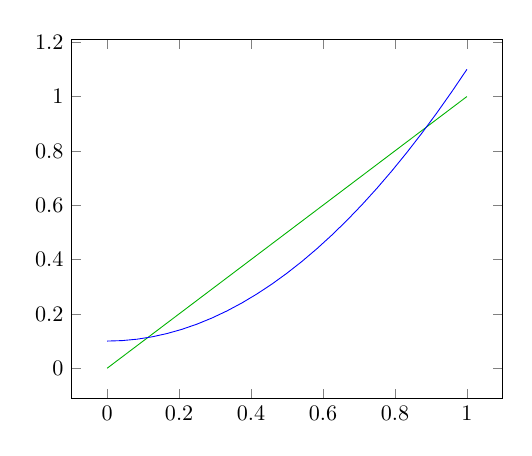
\begin{tikzpicture}[scale=0.8]
    \begin{axis}[domain=0:1]
      \addplot[green!70!black] {x};
      \addplot[blue] {x^2+0.1};
    \end{axis}
  \end{tikzpicture}
  \quad
  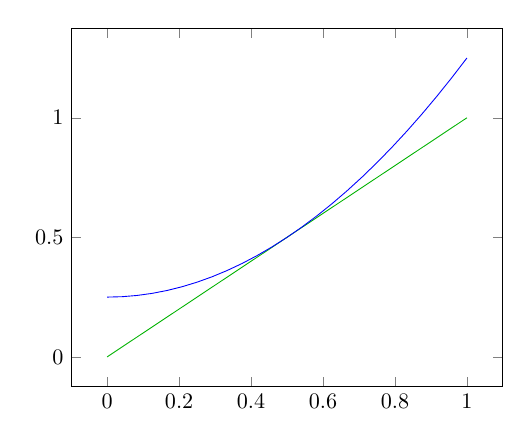
\begin{tikzpicture}[scale=0.8]
    \begin{axis}[domain=0:1]
      \addplot[green!70!black] {x};
      \addplot[blue] {x^2+0.25};
    \end{axis}
  \end{tikzpicture}
  \quad
  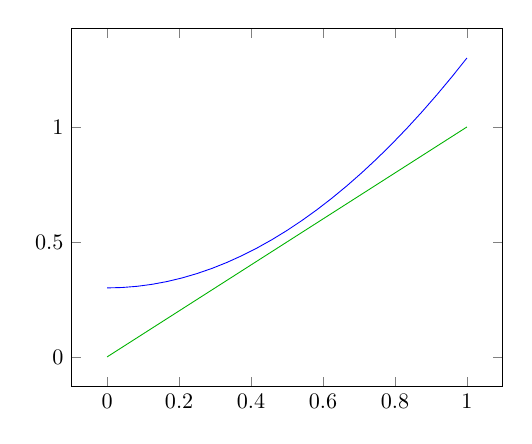
\begin{tikzpicture}[scale=0.8]
    \begin{axis}[domain=0:1]
      \addplot[green!70!black] {x};
      \addplot[blue] {x^2+0.3};
    \end{axis}
  \end{tikzpicture}
\end{center}
for $\lambda<\lambda_0$, $\lambda = \lambda_0$, and $\lambda > \lambda_0$.

\begin{example}
  Consider the exponential family $E_\lambda(x) = e^x + \lambda$ at $\lambda_0=-1$.
\end{example}

This is a tangent bifurcation.

\begin{example}
  $F_\lambda(x) = \lambda x(1-x), \lambda_0 = 1$
\end{example}

Here, we have two fixed points on one side of $\lambda_0$
and one fixed point on the other.
So this is a bifurcation but not a tangent bifurcation.

\chapter{Cantor set}

Recall the quadratic family $Q_C(x) = x^2+C$ for $C < -2$.
Then, $p_+ = \frac{1+\sqrt{1-4C}}{2} > 2$ and $-p_+ < -2$.
Consider the interval/region $I = [-p_+,p_+]$ and $I\times I$.

Draw the picture of \textcolor{green!70!black}{$y=x$},
\textcolor{blue}{$y=Q_C(x)$}, and the box \textcolor{red}{$I \times I$}:
\begin{center}
  \begin{tikzpicture}
    \begin{axis}[domain=-4:4,xmin=-4,xmax=4,ymin=-4,ymax=4,hide axis]
      \addplot[green!70!black] {x};
      \addplot[blue] {x^2-3};
      \addplot[domain=-0.835:0.835,violet,ultra thick] {x^2-3};
      \draw[red] (2.303,2.303) rectangle (-2.303,-2.303);
    \end{axis}
  \end{tikzpicture}
\end{center}
Let \textcolor{violet}{$J_1 \subseteq I$} be the interval such that $Q_C(x) \not\in I$ for all $x \in J_1$.

For $x \in J_1$, $Q_C^n(x) \to \infty$.
Moreover, if there exists $n$ such that $Q_C^n(x) \in J_1$,
then $Q_C^n(x) \to \infty$.

Consider the set of points $\Lambda = \{x \in I : \forall n, Q_C^n(x) \in I\}$
with ``interesting'' orbits staying inside $I$.

Now, let $J_2 = \{x \in I : Q_C(x) \in J_1\} = \{x \in I : Q_C^2(x) \not\in I\}$
and define higher $J_n$ likewise.

Then, $\Lambda = I \setminus (J_1 \cup J_2 \cup \dotsb)$
is a \term*{Cantor set}, that is, a fractal. {\tiny (roll credits!)}

Drawing $\Lambda$ on the $x$-axis, we get something that looks like
\begin{center}
  \begin{tikzpicture}
    \draw[|-|] (0,0) -- (9,0);
    \draw[(-)] (3,0) -- node[below] {$J_1$} (6,0);
    \draw[(-)] (1,0) -- node[below] {$J_2$} (2,0);
    \draw[(-)] (7,0) -- node[below] {$J_2$} (8,0);
    \draw[(-)] (0.33,0) -- node[below] {$J_3$} (0.67,0);
    \draw[(-)] (2.33,0) -- node[below] {$J_3$} (2.67,0);
    \draw[(-)] (6.33,0) -- node[below] {$J_3$} (6.67,0);
    \draw[(-)] (8.33,0) -- node[below] {$J_3$} (8.67,0);
  \end{tikzpicture}
\end{center}

\textrule{$\downarrow$ Lecture 9 adapted from Imaad $\downarrow$}
\lecture{Jan 26}

\begin{defn*}[Cantor middle thirds set]\label{def:cantor}
  Let $C_0 = [0,1]$. Remove the open middle third interval each time.

  That is, $C_1 = [0,\frac13] \cup [\frac23,1]$,
  $C_2 = [0,\frac19] \cup [\frac29,\frac13] \cup [\frac23,\frac79] \cup [\frac89,1]$,
  and so on.

  The set $K = \bigcap_{n=1}^\infty C_n$ is the \term[Cantor set]{Cantor (middle thirds) set}.
\end{defn*}

\begin{prop}
  Suppose a bunch of sets $A_n \subseteq \R$ are closed.
  Then, $\bigcap A_n$ is also closed.
\end{prop}
\begin{prf}
  Let $(a_k) \subseteq \cap A_n$ where $(a_k) \to a$.

  Note that for all $n$, $(a_k) \subseteq A_n \implies a \in A_n \implies a \in \bigcap A_n$
\end{prf}

\begin{prop}
  Let $A,B \subseteq \R$ be closed.
  Then, $A \cup B$ is closed.
\end{prop}
\begin{prf}
  Let $(a_n) \subseteq A \cup B$ where $a_n \to a$.

  \WLOG, $\{n : a_n \in A\}$ is infinite.
  This allows us to construct $(b_n) \subseteq A$ such that $b_n \to a$.

  Since $A$ is closed, $a \in A \subseteq A \cup B$.
\end{prf}

\begin{theorem}[Cantor sets are closed]
  Any Cantor set, in particular $K$, is closed.
\end{theorem}

\begin{theorem}
  $K$ contains no non-empty open intervals.
\end{theorem}
\begin{prf}
  Consider $I \subseteq K$. Then $\forall n, I \subseteq C_n$.

  Then $\ell(I) \leq \frac{1}{3^n} \implies \ell(I)=0 \implies I=\varnothing$, contradiction.
\end{prf}

Now, let's consider the base-3 expansion of $x \in [0,1]$.
$x=0.s_1s_2s_3, \cdots, s_i \in \{0, 1, 2\}$

Consider $\underbrace{[0,1/3]}_{s_1=0}$ and $\underbrace{[2/3, 1]}_{s_1=2}$ and
$\underbrace{[0, 1/9]}_{s_1=0, s_2=0} \ [2/9, 1/3] \ [2/3, 7/9] \ [8/9, 1]$.

\begin{remark}\label{rem:ternary}
  $x \in K$ if and only if $x$ can be written in base 3 using only 0s and 2s
\end{remark}

\begin{example}
  $\frac{1}{3} \in K$. $\frac{1}{3} = 0.1_3 = 0.02222\dots_3$
\end{example}

\begin{theorem}
  $K$ is uncountable and $\abs{K} = \abs{\R}$.
\end{theorem}

\textrule{$\uparrow$ Lecture 9 adapted from Imaad $\uparrow$}

\chapter{Symbolic dynamics}
\lecture{Jan 29}

Recall the construction of the Cantor set from the quadratic family:
\begin{quote}
  Fix $C < -2$ and consider $Q_C(x) = x^2 + C$.
  Define an interval $I = [-p_+,p_+]$
  for a fixed point $p_+ = \frac{1+\sqrt{1-4C}}{2}$.
  Then, let
  \begin{align*}
    J_1 & = \{x \in I : Q_C(x) \not\in I\} \\
    J_2 & = \{x \in I : Q_C(x) \in J_1\}   \\
    J_3 & = \{x \in I : Q_C(x) \in J_2\}   \\
        & \vdotswithin{=}
  \end{align*}
  and define $\Lambda = I \setminus (\bigcup J_i) = \{x \in I : \forall n, Q^n_C(x) \in I\}$.
\end{quote}
We proceed to do some analysis of $\Lambda$ by translating into
some sort of sequence space, doing analysis, and then going back to the Cantor set.

\begin{notation}
  Define closed intervals $I_0 \cup I_1 := I \setminus J_1$ on the left/right of $J_1$:
  \begin{center}
    \begin{tikzpicture}
      \draw[|-|] (0,0) -- (9,0);
      \draw[(-)] (3,0) -- node[below] {$J_1$} (6,0);
      \draw[{[-]}] (0,0) -- node[below] {$I_0$} (3,0);
      \draw[{[-]}] (6,0) -- node[below] {$I_1$} (9,0);
    \end{tikzpicture}
  \end{center}
\end{notation}

\begin{defn}
  For $x \in \Lambda$, the \term{itinerary} of $x$ is
  the sequence $S(x) = (x_0x_1x_2x_3\cdots)$ with $x_i \in \{0,1\}$
  where $x_i = 0 \iff Q_C^i(x) \in I_0$
  and $x_i = 1 \iff Q_C^i(x) \in I_1$.
\end{defn}

Our goal is to understand $S(x)$ better so that we can glean information about $\Lambda$.

\begin{notation}
  Let $\Sigma = \{(x_0x_1x_2\cdots) : x_i \in \{0,1\}\}$ be the sequence space.
  Write elements of $\Sigma$ as binary strings.
  Then, $S : \Lambda \to \Sigma$ is a function.
\end{notation}

It would be helpful to define some PMATH 351/topology shit.

\section{Intro to topology}

\begin{defn}[metric space]
  Let $X$ be a set.
  A function $d : X \times X \to [0,\infty)$ is a \term{metric} if
  \begin{enumerate}[nosep]
    \item $d(x,y) = 0 \iff x = y$ (positive definiteness),
    \item $d(x,y) = d(y,x)$ (symmetry), and
    \item $d(x,y) \leq d(x,z) + d(z,y)$ (triangle inequality).
  \end{enumerate}
  The pair $(X,d)$ is a \term{metric space}.
\end{defn}

Once we have a metric space with a notion $d$ of distance,
we can adapt all our definitions from real analysis to an abstract space.

\begin{example}
  The following are all metrics:
  \begin{itemize}
    \item $X = \R$, $d(x,y) = \abs{x-y}$
    \item $X = \R^n$, $d(\x, \y) = \sqrt{(x_1-y_1)^2 + \dotsb + (x_n-y_n)^2}$
    \item For any set $X$, the discrete metric $d(x,y) = [x\neq y]$
          (but is not particularly useful).
    \item For a subset $A \subseteq R$, $d(x,y) = \abs{x-y}$ is a metric.
  \end{itemize}
\end{example}

Extremely helpfully, we can define a metric on the sequence space.

\begin{defn}[Cantor space]
  Let $X = \Sigma$.
  Define $d(x,y) = \sum_{i=0}^\infty 2^{-i}\abs{x_i-y_i}$.

  This is well-defined (converges) since $\abs{x_i-y_i} \leq 1$ and $\sum 2^{-i}$ converges.
\end{defn}

\begin{example}
  Let $x = (1111\cdots)$ and $y = (1010\cdots)$.
  Calculate $d(x,y)$.
\end{example}
\begin{sol}
  By definition,
  \begin{align*}
    d(x,y) & = \sum_{i=0}^\infty \frac{x_i-y_i}{2^i}                                                \\
           & = \sum_{i=0}^\infty \frac{1}{2^{2i+1}} \tag{even indices cancel}                       \\
           & = \frac12\sum_{i=0}^\infty \frac{1}{4^i}                                               \\
           & = \frac12\qty(\frac{1}{1-\frac14}) = \frac12\qty(\frac43) = \frac46 = \frac23 \qedhere
  \end{align*}
\end{sol}

We don't want to do this manual calculation every time.

\begin{prop}\label{prop:bsd}
  Let $x,y \in \Sigma$.
  \begin{enumerate}[nosep]
    \item If $x_i = y_i$ for $i \leq n$, then $d(x,y) \leq \frac{1}{2^n}$.
    \item If $d(x,y) < \frac{1}{2^n}$, then $x_i = y_i$ for $i \leq n$.
  \end{enumerate}
\end{prop}
\begin{prf}
  Suppose $x_i = y_i$ for $i \leq n$.
  Then, $d(x,y) \leq \sum_{k=n+1}^\infty \frac{1}{2^k}$
  since the first $n$ terms will be 0 and $\abs{x_i-y_i} \leq 1$.
  That is, $d(x,y) \leq \frac{1/2^{n+1}}{1-\frac12} = \frac{1}{2^n}$.

  Conversely, suppose $d(x,y) < \frac{1}{2^n}$
  and for a contradiction that there exists $k \leq n$ where $x_k \neq y_k$.
  Then, there will be a $\frac{1}{2^k}$ term in the sum,
  so $d(x,y) \geq \frac{1}{2^k} \geq \frac{1}{2^n}$. Contradiction.
\end{prf}

\begin{example}
  Let $x = (0000\cdots)$ and $y = (1000\cdots)$.
  Then, the distance is $\frac{1}{2^0} = 1$.
  However, $x_0 \neq y_0$.
\end{example}

\begin{defn}[shift map]
  The map $\sigma : \Sigma \to \Sigma : (x_0x_1x_2\cdots) \mapsto (x_1x_2x_3\cdots)$
  that shifts a bitstring one bit to the left.
\end{defn}

\begin{remark}
  $\sigma^k(x_0x_1x_2\cdots) = x_k x_{k+1}x_{k+2} \cdots$
\end{remark}

\lecture{Jan 31}
\begin{defn*}[continuity in metric spaces]
  Suppose $(X,d)$ and $(Y,d')$ are (possibly distinct) metric spaces.

  A function $f : X \to Y$ is \term[metric space!continuity]{continuous at $y \in X$}
  if for all $\varepsilon > 0$, there exists a $\delta > 0$
  such that for all $x \in X$,
  \[ d(x,y) < \delta \implies d'(f(x),f(y)) < \varepsilon \]

  We say $f$ is \term*{continuous} if it is continuous at every $y \in X$
\end{defn*}

\begin{prop}
  The shift map $\sigma : \Sigma \to \Sigma$ is continuous.
\end{prop}
\begin{prf}
  Fix $y = (y_0y_1y_2\cdots) \in \Sigma$ and let $\varepsilon > 0$.
  Take $n \in \N$ such that $\frac{1}{2^n} < \varepsilon$.

  Consider $\delta = \frac{1}{2^{n+1}}$.
  Let $x = (x_0x_1x_2\cdots) \in \Sigma$ such that $d(x,y) < \delta$.

  Therefore, by \cref{prop:bsd}, $x_i = y_i$ for $i = 0,1,\dotsc,n+1$.
  Then, $\sigma(x) = (x_1x_2x_3\cdots)$ and $\sigma(y) = (y_1y_2y_3\cdots)$
  agree for the first $n$ terms.

  Again by \cref{prop:bsd}, $d(\sigma(x),\sigma(y)) \leq \frac{1}{2^n} < \varepsilon$.
\end{prf}

\begin{defn*}[convergence in metric spaces]
  Let $(X,d)$ be a metric space, $(x_n) \subseteq X$, and $x \in X$.

  We say $(x_n)$ \term[metric space!convergence]{converges to $x$}
  ($x_n \to x$) if for all $\varepsilon > 0$, there exists $N \in \N$
  such that \[ n \geq N \implies d(x_n,x) < \varepsilon. \]
\end{defn*}

\begin{prop}[sequential characterization of continuity in metric spaces]
  Let $(X,d)$ and $(Y,d')$ be metric spaces and $f : X \to Y$.
  Then, $f$ is continuous if and only if $f(x_n) \to f(x)$
  whenever $x_n \to x$.
\end{prop}

\begin{defn}[homeomorphism]
  Let $(X,d)$ and $(Y,d')$ be metric spaces.
  A function $f : X \to Y$ is a \term{homeomorphism} if
  \begin{enumerate}[nosep]
    \item $f$ is injective,
    \item $f$ is surjective,
    \item $f$ is continuous, and
    \item $f^{-1}$ is continuous.
  \end{enumerate}
\end{defn}

Suppose $f : X \to Y$ is a homeomorphism.
Then, if $(x_n) \subseteq X$ with $x_n \to x$,
then $f(x_n) \to f(x)$.

Likewise, suppose $(y_n) \subseteq Y$ with $y_n \to y$.
Say $y_n = f(x_n)$ and $y = f(x)$.
Then, $f(x_n) \to f(x)$,
so $f^{-1}(f(x_n)) \to f^{-1}(f(x))$
and $x_n \to x$.

That is, $f$ is a \emph{relabelling} of $X$ to $Y$.
We think of $X$ and $Y$ as the ``same metric space''.

\section{Revisiting the itinerary}

\begin{remark}
  Suppose we have $x \in \Lambda$ with $S(x) = (x_0x_1\cdots)$.
  Then, by definition, $x \in I_{x_0}$, $Q_c(x) \in I_{x_1}$, $Q_c^2(x) \in I_{x_2}$, etc.
  Therefore, $S(Q_c(x)) = (x_1x_2\cdots) = \sigma(S(x))$.

  Iterating, $S(Q_c^n(x)) = \sigma^n(x)$.
\end{remark}

\begin{theorem}\label{thm:Shom}
  $S: \Lambda \to \Sigma$ is a homeomorphism.
\end{theorem}

We will prove this with some more tools. Recall from MATH 137:

\begin{theorem}[monotone convergence theorem]\label{thm:mct}
  If $(a_n) \subseteq \R$ is increasing/decreasing and bounded,
  then $(a_n)$ converges.
\end{theorem}

Instead of using this directly, we use a lemma:

\begin{lemma}[nested intervals lemma]\label{lem:nil}
  If $I_1 \supseteq I_2 \supseteq I_3 \supseteq \cdots$ are closed intervals,
  then $\bigcap_{i=1}^\infty I_n \neq \varnothing$.
\end{lemma}
\begin{prf}
  Let $I_k = [a_k, b_k]$.

  That is, $[a_1,b_1] \supseteq [a_2,b_2] \supseteq [a_3,b_3] \cdots$.

  Then, $(a_n)$ is increasing and $(a_n) \subseteq [a_1,b_1]$.
  Likewise, $(b_n)$ is decreasing and $(b_n) \subseteq [a_1,b_1]$.
  By the \nameref{thm:mct}, $a_n \to a$ and $b_n \to b$ for some limit points $a$ and $b$.

  Therefore (handwavey), $\varnothing \neq [a,b] \subseteq \bigcap_{n=1}^\infty I_n$.
\end{prf}

\lecture{Feb 2}
We will now prove \cref{thm:Shom}.
It is true for $c < -2$, but we will show it for $c < -\frac{5+2\sqrt5}{4}$.

\begin{prf}
  (injective) Suppose $x,y \in \Lambda$ with $S(x) = S(y)$ but $x \neq y$.
  Then, for all $n$, $Q_c^n(x)$ and $Q_c^n(y)$ live in the same $I_0$ or $I_1$.
  Recall from Assignment 2 that for all $x \in I \setminus J_1 = I_0 \cup I_1$,
  we have $\abs{Q_c'(x)} \geq \mu > 1$.
  By the mean value theorem,
  \[ \abs{Q_c(x) - Q_c(y)} \geq \mu\abs{x-y}. \]
  Since $Q_c$ is injective on $I_0$ and $I_1$,
  we have that $Q_c(x) \neq Q_c(y)$. Thus,
  \begin{align*}
    \abs{Q^2_c(x) - Q_c^2(y)} & \geq \mu^2\abs{x-y} \\
                              & \vdotswithin{\geq}  \\
    \abs{Q^n_c(x) - Q_c^n(y)} & \geq \mu^n\abs{x-y}
  \end{align*}
  Since $\mu > 1$, we have $\mu^n\abs{x-y} \to \infty$.
  However, $\abs{Q_c^n(x) - Q_c^n(y)} \leq \max\{\ell(I_0),\ell(I_1)\}$,
  so it cannot blow up to infinity.
  Contradiction, so we have injectivity.

  (surjective) Let $y = (y_0y_1\cdots) \in \Sigma$.
  For $n \in \N$, define
  \[ I_{y_0y_1\cdots y_n} := \{x \in I : x \in I_{y_0}, Q_c(x) \in I_{y_1}, \dotsc, Q_c^n(x) \in I_{y_n}\}. \]
  It is enough to show there exists
  \[ x \in \bigcap_{n=1}^\infty I_{y_0y_1\cdots y_n} \]
  which would imply $S(x) = y$.
  Clearly, by definition, $I_{y_0} \supseteq I_{y_0y_1} \supseteq I_{y_0y_1y_2} \supseteq \dotsb$

  We claim that each $I_{y_0y_1\cdots y_n}$ is a closed interval.
  Proceed by induction.

  First, $I_{y_0} \in \{I_0,I_1\}$ so it is closed.
  Assume $I_{y_0y_1\cdots y_n}$ is closed for some $n \geq 0$.
  Note:
  \begin{align*}
         & x \in I_{y_0y_1\cdots y_{n+1}}                                                                                             \\
    \iff & x \in I_{y_0}, Q_c(x) \in I_{y_1}, Q_c(Q_c(x)) \in I_{y_2}, Q_c(Q_c^2(x)) \in I_{y_3},\dotsc,Q_c(Q_c^n(x)) \in I_{y_{n+1}} \\
    \iff & x \in I_{y_0} \cap Q_c^{-1}(I_{y_1y_2\cdots y_{n+1}}) \tag{$\star$}
  \end{align*}
  By the inductive hypothesis, $I_{y_1y_2\cdots y_{n+1}}$ is a closed interval (the subscript has length $n$).

  We have
  \begin{center}
    \begin{tikzpicture}
      \begin{axis}[domain=-4:4,xmin=-4,xmax=4,ymin=-4,ymax=4,hide axis]
        \addplot[dotted,green!70!black] {x};
        \addplot[dotted,blue] {x^2-3};
        \addplot[domain=-2.303:-0.835,blue] {x^2-3} node[above,pos=0] {$I_0$};
        \addplot[domain=0.835:2.303,blue] {x^2-3} node[above,pos=1] {$I_1$};
        \addplot[domain=-2.121:-1.414,purple,ultra thick] {x^2-3};
        \addplot[domain=1.414:2.121,purple,ultra thick] {x^2-3};
        \addplot[orange] {1.5};
        \addplot[orange] {-1};
        \draw[red,dotted] (2.303,2.303) rectangle (-2.303,-2.303);
        \draw[orange,decorate,decoration=brace] (-3,-1) -- node[midway,left,orange]{\rotatebox{90}{$I_{y_1y_2\cdots y_{n+1}}$}} (-3,1.5);
      \end{axis}
    \end{tikzpicture}
  \end{center}
  That is, $Q_c^{-1}(\textcolor{orange}{I_{y_1y_2\cdots y_{n+1}}})$
  is a union of \textcolor{purple}{two disjoint closed intervals}, one in $I_0$ and one in $I_1$.

  In particular, returning to ($\star$),
  $I_{y_0y_1\cdots y_{n+1}} = I_{y_0} \cap Q_c^{-1}(I_{y_1y_2\cdots y_{n+1}})$
  is one of these closed intervals.

  By the \nameref{lem:nil}, there must exist $x \in \bigcap_{n=1}^\infty I_{y_0y_1\cdots y_n}$.
  Hence, $S(x) = y$ and we have surjectivity.

  (continuous) Fix $y \in \Lambda$ and say $S(y) = (y_0y_1y_2\cdots)$.
  Let $\varepsilon > 0$ and choose $n$ such that $\frac{1}{2^n} < \varepsilon$.

  Consider the $2^{n+1}$ disjoint, closed intervals $I_{t_0t_1\cdots t_n}$.

  Pick $\delta > 0$ such that $(y-\delta,y+\delta)$ only overlaps with $I_{y_0y_1\cdots y_n}$.
  We know $\delta$ exists since we have a finite set of disjoint closed intervals.

  For $x \in \Lambda$ with $\abs{x-y} < \delta$,
  $x \in I_{y_0y_1\cdots y_n}$ and so $d(S(x), S(y)) \leq \frac{1}{2^n} < \varepsilon$.

  (continuous inverse) Similar.
\end{prf}

\chapter{Chaos}
\lecture{Feb 5}

\section{Prerequisites to chaos}

\begin{defn}[density]
  Let $(X,d)$ be a metric space.
  We say $A \subseteq X$ is \term*{dense in $X$}
  if for all $x \in X$ and $\varepsilon > 0$,
  there exists $a \in A$ such that $d(a,x) < \varepsilon$.
\end{defn}

Informally, there is always something ``that close'' to any point.

\begin{example}
  $\Q$ is dense in $\R$.
  Given a real number, there is always a decimal approximation with arbitrary accuracy.

  $\Z$ is not dense in $\R$.
  Given $x = \frac12 \in \R$, there are no integers within $\varepsilon = \frac14$.
\end{example}

\begin{example}
  Let $A = \{x \in \Sigma : \exists N, \forall i > N, x_i = 0\}$,
  i.e., the sequences which are eventually constant 0s.
  This is dense in $\Sigma$.
\end{example}
\begin{prf}
  Let $x = (x_0x_1x_2\cdots) \in \Sigma$ and let $\varepsilon > 0$.
  As usual, take $n \in \N$ such that $\frac1{2^n} < \varepsilon$.

  Consider $y = (x_0x_1x_2\cdots x_n0000\cdots) \in A$.
  Then, by \cref{prop:bsd}, $d(x,y) \leq \frac{1}{2^n} < \varepsilon$.
\end{prf}

\begin{xca}\label{xca:dense}
  Let $A = \{x \in \Sigma : \text{$x$ is periodic}\}$.
  Show that this is dense in $\Sigma$.
\end{xca}

\begin{remark}
  $A$ in \cref{xca:dense} is exactly the set of periodic points for
  the shift map $\sigma : \Sigma \to \Sigma$.
\end{remark}

\begin{prop}\label{prop:Sdense}
  There exists $z \in \Sigma$ such that $\{\sigma^k(z) : K \in \N \cup \{0\}\}$
  is dense in $\Sigma$.
\end{prop}
\begin{prf}
  Take $z = (0\ 1\ 00\ 01\ 10\ 11\ 000\ 001\ \cdots)$
  to contain all possible blocks of increasing sizes.

  Let $x \in \Sigma$ and $\varepsilon > 0$.
  Again, let $\frac{1}{2^n} < \varepsilon$.

  For some $k$, $\sigma^k(z)$ and $x$ agree on the first $n$ terms.
  This must exist because $z$ has \emph{every possible} sequence of $n$ terms.
  That is, by \cref{prop:bsd}, $d(\sigma^k(z),x) \leq \frac1{2^n} < \varepsilon$.
\end{prf}

Warning: \cref{def:dynsys} is not the normal definition from applied math textbooks,
but it is what we will use in the course.

\begin{defn}[dynamical system]
  A metric space $(X,d)$ together with a continuous function $f : X \to X$.
  \label{def:dynsys}
\end{defn}

This is an abstract space in which we can do orbit analysis and all our fun stuff.

\begin{example}
  $\sigma : \Sigma \to \Sigma$ is a dynamical system (see \cref{thm:Shom}).
\end{example}

\begin{defn}[transitivity]
  We say a dynamical system $f : X \to X$ is \term*{transitive}
  if for all $x,y \in X$ and $\varepsilon > 0$,
  there exists $z \in X$ and $n,m \in \N \cup \{0\}$
  such that $d(x,f^n(z)) < \varepsilon$ and $d(y,f^m(z)) < \varepsilon$.
\end{defn}

Informally, given any two points, there is a special point whose orbit
gets arbitrarily close to both points.

\begin{prop}\label{prop:Strans}
  $\sigma : \Sigma \to \Sigma$ is transitive.
\end{prop}
\begin{prf}
  Take $z$ from \cref{prop:Sdense} such that the orbit is dense in $\Sigma$.

  Then, for all $\varepsilon > 0$ and $x,y \in \Sigma$,
  there must exist by the definition of density $n$ and $m$ such that
  $d(x,\sigma^n(z)) < \varepsilon$ and $d(y,\sigma^m(z)) < \varepsilon$.
\end{prf}

\begin{defn*}[sensitive dependence on initial conditions]
  Let $f : X \to X$ be a dynamical system.

  We say $f$ is \term*{sensitively dependent on initial conditions}
  (or just \term{sensitive}) if
  \[ \exists \beta > 0,\ \forall \varepsilon > 0,\ \forall x \in X,\ \exists y \in X,\ \exists k \in \N \]
  such that $d(x,y) < \varepsilon$ and $d(f^k(x),f^k(y)) \geq \beta$.
\end{defn*}

Informally, there exists a ``wrongness'' $\beta$ that can always be
achieved in the orbit no matter how close two starting points are.

\begin{prop}\label{prop:Ssense}
  $\sigma : \Sigma \to \Sigma$ is sensitive.
\end{prop}
\begin{prf}
  Take $\beta = 1$.

  Let $\varepsilon > 0$ and let $x \in \Sigma$.
  Say $\frac1{2^n} < \varepsilon$ and pick $y \in \Sigma$
  such that $0 < d(x,y) < \frac1{2^n}$.
  That is, $x$ and $y$ must agree on the first $n$ terms by \cref{prop:bsd},
  but they are not equal.

  Therefore, there exists $k \geq n$ such that $x_k \neq y_k$.

  In the distance $d(\sigma^k(x),\sigma^k(y)) \geq \frac{\abs{x_k-y_k}}{2^0} \geq 1 = \beta$.
\end{prf}

\section{Defining chaos}
\textrule{$\downarrow$ Lectures 14 and 15 adapted from Imaad $\downarrow$}
\lecture{Feb 7}

\begin{defn}[chaos]
  A dynamical system $f: X \to X$ is \term*{chaotic} if
  \begin{enumerate}[nosep]
    \item the periodic points for $f$ are dense in $X$,
    \item $f$ is transitive, and
    \item $f$ is sensitive.
  \end{enumerate}
\end{defn}

\begin{theorem}
  $\sigma: \Sigma \to \Sigma$ is chaotic.
\end{theorem}
\begin{prf}
  By \cref{prop:Sdense,prop:Strans,prop:Ssense}.
\end{prf}

\begin{prop}\label{prop:dense}
  Let $(X, d), (Y, d')$ be metric spaces.

  Suppose $f: X \to Y$ is continuous and surjective.
  If $A \subseteq X$ is dense in $X$, then $f(A)$ is dense in $Y$.
\end{prop}
\begin{prf}
  Let $y \in Y$ and say $y = f(x)$.

  Let $\epsilon > 0$.
  Since $f$ is continuous at $x$, there exists $\delta > 0$ such that
  \[ d(z, x) < \delta \implies d'(f(z), f(x)) < \epsilon \]
  for any $z$. In particular, since $A$ is dense in $X$, we may find $a \in A$ such that
  \[ d(a, x) < \delta \implies d'(f(a), f(x)) = d'(f(a), y) < \epsilon \]
  as desired.
\end{prf}

\begin{theorem}
  Let $c < \frac{-(5+2\sqrt{5})}{4}$.
  Then, $Q_c: \Lambda \to \Lambda$ is chaotic.
\end{theorem}
\begin{prf}
  (periodic point density)
  Note that $Q_c^n(x)=x \iff S(Q_c^n(x)) = S(x) \iff \sigma^n(S(x)) = S(x)$.

  By \cref{prop:dense} applied to $S^{-1}: \Sigma \to \Lambda$,
  the periodic points for $Q_c$ are dense in $\Lambda$.

  (transitivity)
  Take $z \in \Sigma$ from \cref{prop:Sdense}
  such that $\{\sigma^K(z): K \in \N \cup \{0\}\}$ is dense in $\Sigma$.
  Again by \cref{prop:dense}, $\{S^{-1}(\sigma^K(z)): K \in \N \cup \{0\}\}$
  is dense in $\Lambda$.

  Note: Say $S(x)=z$, we know $(S(Q_c^K(x))) = \sigma^K(S(x))$ $\iff$ $Q_c^K(x) = S^{-1}(\sigma^K(S(x)))$

  This, $\{Q_c^K(x): K \in \N \cup \{0\}\}$ is dense in $\Lambda$.
  As in \cref{prop:Strans}, we have that $Q_c$ is transitive.

  (sensitivity)
  Recall that $\Lambda \subseteq I \setminus J_1 = I_0 \cup I_1$.
  Let $\beta > 0$ be less than the gap between $I_0$ and $I_1$.

  For $x, y \in \Lambda$ with $x \neq y$, supppose $S(x) \neq S(y)$.
  Then, there must exist a $k$ where $k$\xth term of $S(x)$
  does not equal the $k$\xth term of $S(y)$.

  Hence, $|Q_c^k(x) - Q_c^k(y)| > \beta$ and $Q_c$ is sensitive.
\end{prf}

\chapter{Sarkovskii's Theorem}
\lecture{Feb 9}
\begin{theorem}[period 3]\label{thm:p3}
  Let $f: \R \to \R$ be continuous.
  If $f$ has a point with period 3,
  then $f$ has a point with period $n$ for all $n \in \N$.
\end{theorem}

\begin{prop}\label{prop:1}
  Let $I \subseteq J$ be closed intervals and suppose $f: \R \to \R$ is continuous.
  If $f(I) \supseteq J$, then $f(x)$ has a fixed point in $I$.
\end{prop}

\begin{prop}\label{prop:2}
  Let $I, J$ be closed intervals, $f: \R \to \R$ be continuous, and $f(I) \supseteq J$.
  Then, there exists a closed interval $I' \subseteq I$ such that $f(I') = J$.
\end{prop}

We can now prove \cref{thm:p3}.
\begin{prf}
  Let $a \in \R$ be a period 3 point for $f(x)$. Say $f(a)=b, f(b)=c, f(c)=a$.
  \WLOG, suppose $a < b$ and $a < c$.

  Suppose $a < b < c$. The case where $a < c < b$ is left as an exercise.

  Let $I = [a, b]$ and $J = [b, c]$.
  Then, $f(a)=b$ and $f(b)=c$ imply by IVT that $[b,c] = J \subseteq f(I)$.
  Likewise, $f(b)=c$ and $f(c)=a$ imply by IVT that $[a,c] = I \cup J \subseteq f(J)$.

  Since $J \subseteq f(J)$, there exists a closed interval $A_1 \subseteq J$
  such that $f(A_1) = J$ by \cref{prop:2}.
  Again, $A_1 \subseteq J = f(A_1)$,
  so there exists a closed interval $A_2 \subseteq A_1$ such that $f(A_2)=A_1$.

  Now, fix $n > 3$.
  Repeating the above process,
  we can find $A_{n-2} \subseteq A_{n-3} \subseteq \dotsb \subseteq A_2 \subseteq A_1 \subseteq J$
  such that $f(A_i) = A_{i-1}$.
  Now, $f(I) \supseteq J \supseteq A_{n-2}$ means there exists a closed interval
  $A_{n-1} \subseteq I$ such that $f(A_{n-1}) = A_{n-2}$.

  Moreover, $f(J) \supseteq I \supseteq A_{n-1}$
  which means there exists a closed interval $A_n \subseteq J$
  such that $f(A_n)=A_{n-1}$.

  We have $f^n(A_n)=J$ and $A_n \subseteq J$.
  By \cref{prop:1}, there exists $x_0 \in A_n$ such that $f^n(x_0)=x_0$.

  Note: for $x_0 \in A_n$, $f(x_0) \in A_{n-1} \subseteq I$, $f^i(x_0) \in J$ for $i=2, 3, \dotsc, n$.

  For contradiction, suppose $f^i(x_0)=x_0$ for $i < n$.

  Then, $\overbrace{f(x_0)}^{\in I} = \overbrace{f^{i+1}(x_0)}^{\in J} = b$
  so $f(x_0) = b$, $f^2(x_0)=c$, and $f^3(x_0) = a$,
  which is a contradiction because $f^3(x_0) \in J$ but $a \not\in J$.
  Hence, $x_0$ has period $n$.

  That is, $f$ has a periodic point with period $n$ for all $n > 3$.

  Further, $f(J) \supseteq J$ and so by \cref{prop:1},
  $f$ has a fixed point (aka period 1) in $J$.

  Finally, $f(I) \supseteq J$ means $J=f(I')$ and $f(J) \supseteq I'$ means $f(J')=I'$.
  This implies $f^2(j') = f(I') = J \sup J'$.
  Therefore, we know there exists $x \in J'$ such that $f^2(x)=x$.

  If $f(x)=x$, then $x \in J'$ and $f(x) \in I'$, meaning $x=b$.
  But, $f(b) \neq b = c$, contradiction.

  Hence, $x$ has period 2.

  Therefore, since we already supposed $f$ has a period 3 point,
  $f$ has a period $n$ point for all $n$.
\end{prf}

\begin{xca}
  Complete the proof for the case where $a < c < b$.
\end{xca}

\textrule{$\uparrow$ Lectures 14 and 15 adapted from Imaad $\uparrow$}

\lecture{Feb 12}
Draw the continuous function
\begin{center}
  \begin{tikzpicture}
    \begin{axis}[xmin=-0.5,xmax=6.5,ymin=0.5,ymax=5.5]
      \draw (1,3) -- (2,5) -- (5,1);
      \addplot[domain=-1:1] {3};
      \addplot[domain=5:7] {1};
    \end{axis}
  \end{tikzpicture}
\end{center}
Then, the orbit of 1 is $1 \mapsto 3 \mapsto 4 \mapsto 2 \mapsto 5 \mapsto 1$
and 1 has period 5.

\begin{claim}
  $f$ has no point with period 3.
\end{claim}
\begin{prf}
  Suppose that $f$ has a point $x$ with period 3.
  Then, $1 \leq x \leq 5$.

  Suppose $x \in [1,2]$.
  Then, $x \in [1,2] \cap f^3([1,2])$ since $x = f^3(x)$.
  But $f^3([1,2]) = [2,5]$, so $x = 2$.
  However, 2 has period 5 since it is on the same 5-cycle given above.

  Suppose instead that $x \in [2,3]$.
  Then, $x \in [2,3] \cap f^3([2,3]) = [2,3] \cap [3,5] = \{3\}$
  which is also on the 5-cycle.

  If $x \in [4,5]$, then $x \in [4,5] \cap f^3([4,5]) = [4,5] \cap [1,4] = \{4\}$
  which is, again, on the 5-cycle.

  Finally, suppose that $x \in [3,4]$.
  Then, $f([3,4]) = [2,4]$ and it is strictly decreasing.
  Further, $f([2,4]) = [2,5]$ and it is also strictly decreasing.
  Once more, $f([2,5]) = [1,5]$ and it is again strictly decreasing.
  Since $f^3$ is strictly decreasing, it has a unique fixed point in $[3,4]$,
  but it is just the fixed point of $f$.

  Since we have covered the entire interval $[1,5]$, $x$ must not exist.
\end{prf}

\begin{example}
  The function $f(x) = \begin{cases}
      1 & x < -1 \\ -x & -1 \leq x \leq 1 \\ 1 & x > 1
    \end{cases}$
  has a period 1 point at $x=0$, period 2 points $[-1,1] \setminus \{0\}$,
  and no other periodic points.
\end{example}

\begin{defn}[Sarkovskii ordering]
  Start by ordering the odd numbers $3 \prec 5 \prec 7 \prec 9 \prec \dotsb$

  Then, all those are $\dotsb \prec 2\cdot 3 \prec 2\cdot5 \prec 2\cdot7 \prec \dotsb$

  All those are $\dotsb \prec 2^2\cdot3 \prec 2^2\cdot5 \prec 2^2\cdot7 \prec \dotsb$

  Complete the ordering as $\dotsb \prec 2^n \prec 2^{n-1} \prec \dotsb \prec 2^2 \prec 2 \prec 1$.

  This is a total order on the natural numbers.
\end{defn}

\begin{example}
  \leavevmode
  \begin{itemize}[nosep]
    \item $26 = 2\cdot 13 \prec 2^2\cdot 5 = 40$ because the exponent of 2 is smaller.
    \item $3072 = 2^{10}\cdot 3 \prec 2^5 = 32$ because powers of 2 are big.
    \item $n \preccurlyeq 1$ for all $n$.
    \item $2^{15} \prec 2^3$ since the powers of 2 are ordered backwards.
  \end{itemize}
\end{example}

\begin{theorem}[Sarkovskii's theorem]
  Let $f : \R \to \R$ be continuous.
  Suppose $n \prec m$ in the Sarkovskii ordering.
  Then, if $f$ has a point with period $n$, then it has a point with period $m$.
\end{theorem}

\chapter{Fractals}

\section{Definitions and dimensions}
\lecture{Feb 14}

\begin{defn}
  Define a few things from topology.
  \begin{itemize}[nosep]
    \item For $\x \in \R^n$, the \term{norm} $\norm{\x} = \sqrt{x_1^2+x_2+\dotsb+x_n^2}$
    \item $d(\x,\y) = \norm{\x - \y}$ is our default metric on $\R^n$
    \item For $\x \in \R^n$, $\varepsilon > 0$, the \term{open ball} of radius $\varepsilon$ centered at $x$
          is $B_\varepsilon(\x) = \{\y \in \R^n : \norm{\x - \y < \varepsilon}\}$
    \item We say $U \in \R^n$ is \term{open} if for all $\x \in U$,
          there exists $\varepsilon > 0$ such that $B_\varepsilon(\x) \subseteq U$.
    \item The \term{boundary} $\delta(A)$ of a set $A \subseteq \R^n$
          is the closure of $A$ without the interior of $A$.
  \end{itemize}
\end{defn}

\begin{defn*}[topological dimension (zero case)]
  We say $S \subseteq \R^n$ has \term{topological dimension} $\dim_t S = 0$
  if for all $\x \in S$, there exists arbitrarily small open sets $U \ni \x$
  such that $\delta(U) \cap S = \varnothing$.
\end{defn*}

\begin{example}
  Let $X = \begin{tikzpicture}[scale=0.3]
      \draw[fill=black] (-1,-1) circle (3 pt);
      \draw[fill=black] (0,1) circle (3 pt);
      \draw[fill=black] (1,-1) circle (3 pt);
    \end{tikzpicture}$.
  Then, since we can draw balls
  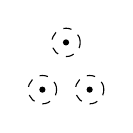
\begin{tikzpicture}[scale=0.3]
    \draw[fill=none,dashed] (-1,-1) circle (0.6);
    \draw[fill=black] (-1,-1) circle (3 pt);
    \draw[fill=none,dashed] (0,1) circle (0.6);
    \draw[fill=black] (0,1) circle (3 pt);
    \draw[fill=none,dashed] (1,-1) circle (0.6);
    \draw[fill=black] (1,-1) circle (3 pt);
  \end{tikzpicture}
  separating each point, $\dim_t X = 0$.
\end{example}

\begin{example}
  $X = \{\frac1n : n \in \N\} \cup \{0\}$
  has topological dimension 0.
\end{example}

\begin{defn*}[topological dimension (non-zero case)]
  A set $S \subseteq \R^n$ has \term{topological dimension} $k \in \N$
  if for all $\x \in S$, there exists arbitrarily small
  $U \ni \x$ such that $\delta(U) \cap S$ has topological dimension $k-1$,
  where $k$ is minimal with this property.
\end{defn*}

\begin{example}
  Consider a line $X = \begin{tikzpicture}
      \draw[fill=black] (0,0) circle (1 pt);
      \draw (0,0) -- (1,0.7);
      \draw[fill=black] (1,0.7) circle (1 pt);
    \end{tikzpicture}$.
  Then, since any ball's boundary
  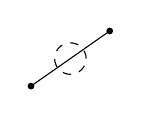
\begin{tikzpicture}
    \draw[fill=black] (0,0) circle (1 pt);
    \draw (0,0) -- (1,0.7);
    \draw[fill=none,dashed] (0.5,0.35) circle (0.2);
    \draw[fill=black] (1,0.7) circle (1 pt);
  \end{tikzpicture}
  creates an intersection made of two distinct points
  (i.e., a set with topological dimension 0),
  we know that $\dim_t X = 1$.
\end{example}

\begin{example}
  Let $X$ be a circle \tikz{\draw[fill=none] (0,0) circle (0.5);}.
  Again, any ball's boundary
  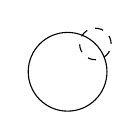
\begin{tikzpicture}
    \draw[fill=none] (0,0) circle (0.5);
    \draw[fill=none,dashed] (0.353,0.353) circle (0.2);
  \end{tikzpicture}
  still only has two intersecting points, so $\dim_t X = 1$.
\end{example}

\begin{example}
  Let $X$ be a filled 2D region.
  \begin{center}
    \begin{tikzpicture}[use Hobby shortcut,closed=true,scale=0.5]
      % [tex.se/603127] stolen blob shape
      \draw[blue,fill=blue!30] (-3.5,0.5) .. (-3,2.5) .. (-1,3.5).. (1.5,3).. (4,3.5).. (5,2.5).. (5,0.5) ..(2.5,-2).. (0,-0.5).. (-3,-2).. (-3.5,0.5);
      \draw[fill=none,orange] (0.353,0.353) circle (0.4);
      \draw[dashed] (-3.5,1) arc(90:270:1);
      \draw[red] (-3.5,-1) arc(-90:90:1);
    \end{tikzpicture}
  \end{center}
  Then, the intersection of a ball's boundary
  will give either a \textcolor{orange}{circle} or an \textcolor{red}{arc},
  which have topological dimension 1,
  so the region has topological dimension 2.
\end{example}

\begin{example}
  Let $X$ be a non-filled sphere.
  \begin{center}
    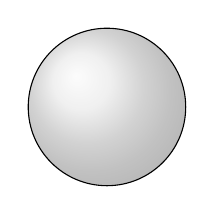
\begin{tikzpicture}
      \shade[ball color = gray!40, opacity = 0.4] (0,0) circle (1cm);
      \draw (0,0) circle (1cm);
    \end{tikzpicture}
  \end{center}
  Then, the intersection of a 3D ball's boundary
  will give a circle, which has topological dimension 1,
  so $\dim_t X = 2$.
\end{example}

\begin{example}
  Let $X$ be a filled sphere.

  Then, a 3D ball's boundary's intersection is either a hollow sphere
  or a spherical cap, which each have topological dimension 2,
  so $\dim_t X = 3$.
\end{example}

\begin{defn}[fractal dimension]
  We say $S \subseteq \R^n$ is \term{self-similar} if $S$ may be divided into
  $K$ congruent subsets, each of which may be magnified by a fixed $M$
  to yield $S$ itself.

  The \term*{fractal dimension} of $S$ is given by $\dim_f S = \frac{\ln K}{\ln M}$.
\end{defn}

\begin{defn}[fractal]
  A \term*{fractal} is a self-similar $S \subseteq \R^n$
  such that $\dim_f S > \dim_t S$.
\end{defn}

\section{Fractal gallery}

\begin{example}
  Let $X = \tikz{
      \draw[fill=black] (0,0) circle (1 pt);
      \draw (0,0) -- (1,0);
      \draw[fill=black] (1,0) circle (1 pt);
    }$ be a line.
  Then, since we can divide it into $n$ smaller lines each of size $\frac1n$,
  it has fractal dimension $\dim_f X = \frac{\ln n}{\ln n} = 1$.
  The topological dimension is $\dim_t X = 1$.

  So this is not a fractal, and is indeed just \term*{boring} (not a fractal).
\end{example}

\begin{example}[Sierpinski triangle]
  Let $X$ be the Sierpinski triangle, i.e., the limiting point of the process:
  \begin{center}
    \multido{\iA=1+1}{4}{%
      \begin{pspicture}(2,1.4)\psSier(0,0){2cm}{\iA}\end{pspicture}\quad}
  \end{center}
  Then, the topological dimension is $\dim_t X = 1$ because,
  in the limit, any ball will touch only single points.
  In particular, we can imagine balls touching the three points of a triangle.

  However, the fractal dimension is
  $\dim_f X = \frac{\ln 3}{\ln 2} \approx 1.58 > 1$
  because each step is consisted of 3 previous steps scaled by $\frac12$.
  so $X$ is a fractal!
\end{example}

\lecture{Feb 16}
\begin{example}[Cantor set]
  Let $K$ be a middle-thirds Cantor set, i.e., the limiting point of the process:
  \begin{center}
    \begin{pspicture}(10,-2)\psCantor\end{pspicture}
  \end{center}
  For any point in the Cantor set, we can find a small empty region around it
  since we keep cutting away from the sides.
  That is, $\dim_t K = 0$. However, $\dim_f K = \frac{\ln 2}{\ln 3} > 0$.
\end{example}

\begin{example}[Koch curve]
  Let $X$ be the Koch curve, where each line segment is replaced by a bump:
  \begin{center}
    \begin{tikzpicture}[decoration=Koch snowflake]
      \draw (0,0) -- (3,0);
      \draw decorate{ (4,0) -- (7,0) };
      \draw decorate{ decorate{ (8,0) -- (11,0) }};
      \draw decorate{ decorate{ decorate{ (12,0) -- (15,0) }}};
    \end{tikzpicture}
  \end{center}
  As a continuous line, intersection with a ball boundary gives points,
  so $\dim_t X = 1$. We have four copies scaled by $\frac13$, so $\dim_t X = \frac{\ln 4}{\ln 3} > 1$.
\end{example}

\begin{example}[box fractal]\label{ex:box}
  Let $X$ be a box fractal, where we delete edge pieces of a 3x3 grid:
  \begin{center}
    \begin{tikzpicture}
      \fill (0,0) l-system [l-system={box fractal, axiom=F+F+F+F, order=0, anchor=south west, step=2cm}];
      \fill (3,0) l-system [l-system={box fractal, axiom=F+F+F+F, order=1, anchor=south west, step=0.67cm}];
      \fill (6,0) l-system [l-system={box fractal, axiom=F+F+F+F, order=2, anchor=south west, step=0.22cm}];
      \fill (9,0) l-system [l-system={box fractal, axiom=F+F+F+F, order=3, anchor=south west, step=0.074cm}];
    \end{tikzpicture}
  \end{center}
  Then, since the squares are solid, we have topological dimension 1
  but fractal dimension $\dim_f X = \frac{\ln 5}{\ln 3} > 1$.
\end{example}

\begin{example}[Minkowski sausage]
  Let $X$ be the Minkowski sausage, where each line segment is replaced by a square wave:
  \begin{center}
    \begin{tikzpicture}[decoration=Koch curve type 2]
      \draw (0,0) -- (3,0);
      \draw decorate{ (4,0) -- (7,0) };
      \draw decorate{ decorate{ (8,0) -- (11,0) }};
      \draw decorate{ decorate{ decorate{ (12,0) -- (15,0) }}};
    \end{tikzpicture}
  \end{center}
  Then, as a continuous line, $\dim_t X = 1$,
  but we have $\dim_f X = \frac{\ln 8}{\ln 4} = \frac32 > 1$.
\end{example}

There is a hidden connection between iterated systems and fractals!
For example, playing around with the website
\href{http://www.shodor.org/interactivate/activities/TheChaosGame/}{http://www.shodor.org/interactivate/activities/TheChaosGame/}
has a process where each iteration moves a point halfway to one of the vertices.

\lecture{Feb 26}
\textrule{...one reading week later...}

Recall the chaos game:
\begin{enumerate}[nosep]
  \item Start with the vertices $(v_1,v_2,v_3)$ of an equilateral triangle.
  \item Pick $p \in_{\symsf{R}} \R^2$.
  \item Pick $v_i \in_{\symsf{R}} \{v_1,v_2,v_3\}$.
  \item Replace $p$ with the midpoint of $p$ and $v_i$.
  \item Iterate.
\end{enumerate}
Where does the orbit of $p$ end up?
Somehow, exactly in the Sierpinski triangle.
Our goal is to formalize this.

\section{Iterated function systems}

Fix some $\p_0 = \mqty[x_0\\y_0]$ and contraction factor $0 < \beta < 1$. Consider
\[
  F : \R^2 \to \R^2 \qc F\qty(\mqty[x\\y]) = \beta\mqty[x-x_0\\y-y_0] + \mqty[x_0\\y_0]
\]
i.e., $F(\vb p) = \beta(\p - \p_0) + \p_0$. Then,
\begin{enumerate}[nosep]
  \item $F(\p_0) = \p_0$
  \item $\norm{F(\p) - F(\p_0)} = \norm{\beta(\p-\p_0)} = \beta\norm{\p-\p_0}$
  \item $\norm{F^n(\p) - \p_0} = \beta^n\norm{\p-\p_0} \to \vb 0$ so $F^n(\p) \to \p_0$
\end{enumerate}

\begin{defn}
  Let $0 < \beta < 1$ and $\p_1,\dotsc,\p_n \in \R^2$. For each $i = 1,\dotsc,n$, let
  \[ F_i(\p) = \beta(\p-\p_i) + \p_i \]
  Then, $\{F_1,\dotsc,F_n\}$ is an \term{iterated function system} (IFS).

  Fix $\q_0 \in \R^2$. Randomly select an $F_i$. Let $\q_1 = F_i(\q_0)$. Repeat.
  The set of points in which the orbit $\q_1,\q_2,\q_3,\dotsc$ lives
  is the \term{attractor} for the IFS.
\end{defn}

\begin{example}
  Formalize the chaos game. Let $\p_1 = v_1$, $\p_2 = v_2$, $\p_3 = v_3$, and $\beta = \frac12$.
  Then, $F_i(\p) = \frac12(\p-\p_i) + \p_i = \frac12(\p+\p_i)$ is the midpoint.

  The set $\{F_1,F_2,F_3\}$ is an iterated function system whose attractor
  is the Sierpinski triangle.
\end{example}

Note that we can construct pathologically unlucky sequences of $F_i$'s
that give us point sequences that never reach the attractor.
However, we ignore those :)

\begin{example}
  Let $\p_0 = (0,0)\trans$, $\p_1 = (1,0)\trans$, $\p_2 = (0,1)\trans$,
  $\p_3 = (1,1)\trans$, $\p_4 = (\frac12,\frac12)\trans$, and $\beta = \frac13$.

  What fractal does this produce?
\end{example}
\begin{sol}
  Draw the points:
  \begin{center}
    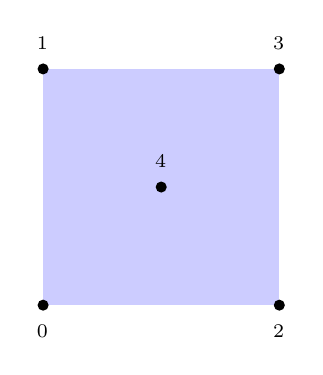
\begin{tikzpicture}
      \fill[blue!20] (0,0) rectangle (3,3);
      \fill (0,0) circle [radius=2pt] node [label=below:{$\p_0$}] {};
      \fill (0,3) circle [radius=2pt] node [label={$\p_1$}] {};
      \fill (3,0) circle [radius=2pt] node [label=below:{$\p_2$}] {};
      \fill (3,3) circle [radius=2pt] node [label={$\p_3$}] {};
      \fill (1.5,1.5) circle [radius=2pt] node [label={$\p_4$}] {};
    \end{tikzpicture}
  \end{center}
  Divide the square into thirds (since we are using $\beta=\frac13$).
  Then, colour in the images of the square under each $F_i$:
  \begin{center}
    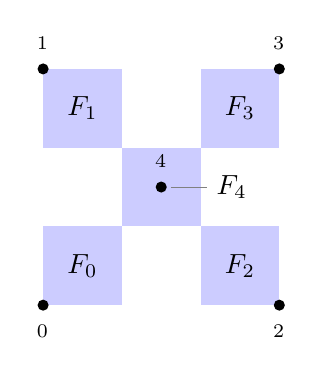
\begin{tikzpicture}
      \fill[blue!20] (0,0) rectangle (1,1) node[black,pos=0.5] {$F_0$};
      \fill[blue!20] (0,3) rectangle (1,2) node[black,pos=0.5] {$F_1$};
      \fill[blue!20] (3,0) rectangle (2,1) node[black,pos=0.5] {$F_2$};
      \fill[blue!20] (3,3) rectangle (2,2) node[black,pos=0.5] {$F_3$};
      \fill[blue!20] (1,1) rectangle (2,2) node[pos=0.5,pin={[black]right:$F_4$}] {};
      \fill (0,0) circle [radius=2pt] node [label=below:{$\p_0$}] {};
      \fill (0,3) circle [radius=2pt] node [label={$\p_1$}] {};
      \fill (3,0) circle [radius=2pt] node [label=below:{$\p_2$}] {};
      \fill (3,3) circle [radius=2pt] node [label={$\p_3$}] {};
      \fill (1.5,1.5) circle [radius=2pt] node [label={$\p_4$}] {};
    \end{tikzpicture}
  \end{center}
  This is going to produce the \nameref{ex:box}.
\end{sol}

\begin{example}
  Repeat with $\p_0 = (0,0)\trans$, $\p_1 = (1,0)\trans$, $\p_2 = (0,1)\trans$,
  and $\beta = \frac12$.
\end{example}
\begin{sol}
  Again, draw the points:
  \begin{center}
    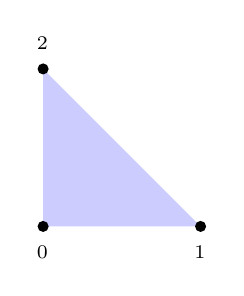
\begin{tikzpicture}
      \fill[blue!20] (0,0) -- (2,0) -- (0,2) -- cycle;
      \fill (0,0) circle [radius=2pt] node [label=below:{$\p_0$}] {};
      \fill (2,0) circle [radius=2pt] node [label=below:{$\p_1$}] {};
      \fill (0,2) circle [radius=2pt] node [label={$\p_2$}] {};
    \end{tikzpicture}
  \end{center}
  Shrink the right triangle by a factor of $\beta = \frac12$ around each point:
  \begin{center}
    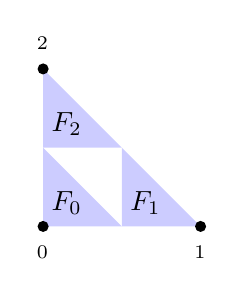
\begin{tikzpicture}
      \fill[blue!20] (0,0) -- (1,0) -- (0,1) -- cycle;
      \fill[blue!20] (0,2) -- (0,1) -- (1,1) -- cycle;
      \fill[blue!20] (1,0) -- (1,1) -- (2,0) -- cycle;
      \node at (0.3,0.3) {$F_0$};
      \node at (0.3,1.3) {$F_2$};
      \node at (1.3,0.3) {$F_1$};
      \fill (0,0) circle [radius=2pt] node [label=below:{$\p_0$}] {};
      \fill (2,0) circle [radius=2pt] node [label=below:{$\p_1$}] {};
      \fill (0,2) circle [radius=2pt] node [label={$\p_2$}] {};
    \end{tikzpicture}
  \end{center}
  This will generate a Sierpinski-like triangle.
\end{sol}

\lecture{Feb 28}
\begin{example}
  Let $\p_0 = (0,0)\trans$, $\p_1 = (1,0)\trans$, $\beta = \frac13$.
  Repeat.
\end{example}
\begin{sol}
  Write the functions explicitly
  \[
    F_0(\x) = \frac13\mqty[x\\y] = \mqty[\frac13x\\\frac13y]
    \qq{and}
    F_1(\x) = \frac13\mqty[x-1\\y] + \mqty[1\\0] = \mqty[\frac13x + \frac23\\\frac13y]
  \]
  and pick a point $\q_0 = (x_0,y_0)\trans \in \R^2$.
  We say that the orbit of $q_0$ under $\{F_0,F_1\}$
  is $q_0,q_1,q_2,\dotsc$ with random selections $s_1,s_2,s_3,\dotsc \in \{0,1\}$
  where $q_i = F_{s_i}(q_{i-1})$.

  First, notice that no matter which one we choose, $y_i = \frac13y_{i-1}$.
  Therefore, $y_n = \frac{1}{3^n}y_0 \to 0$.

  For the $x$-coordinate, we can write it out explicitly to find the pattern:
  \begin{align*}
    x_1 & = \frac13x_0 + \frac{2s_1}{3}                                                          \\
    x_2 & = \frac{1}{3^2}x_0 + \frac{2s_1}{3^2} + \frac{2s_2}{3}                                 \\
        & \vdotswithin{=}                                                                        \\
    x_n & = \frac{1}{3^n}x_0 + \frac{2s_1}{3^n} + \frac{2s_2}{3^{n-1}} + \dotsb + \frac{2s_n}{3}
  \end{align*}
  As $n \to \infty$, the first term disappears.
  The remaining term looks like a funny ternary expansion.
  Therefore, $x_n$ gets arbitrarily close to points of the form
  $\sum_{i=1}^\infty \frac{t_i}{3^i}$ where $t_i \in \{0,2\}$.

  However, the set of points whose ternary expansion uses only 0s and 2s
  is exactly the Cantor set from \cref{def:cantor} (see \cref{rem:ternary}).

  Therefore, the attractor of the IFS $\{F_0,F_1\}$
  is $\{(x,0)\trans : x \in \text{Cantor set}\}$.
\end{sol}

\section{Generated iterated function systems}

We want to generalize our definition of IFSs and fractals
so that we can play with things that look exactly like fractals
(for example, where the scaling factor differs for each piece).

\begin{defn}[affine transformation]
  A function $F : \R^n \to \R^n$ given by $F(\x) = A\x + \vb b$
  where $A \in M_n(\R)$ and $\vb b \in \R^n$.
  If $\vb b = \vb 0$, we recover the linear transformations.

  We call $F$ a \term{linear contraction} if there exists $0 < \lambda < 1$
  such that $\norm{F(\x) - \F(\y)} < \lambda\norm{\x - \y}$.
\end{defn}

In general, ``affine'' just means linear but shifted.

\begin{example}
  Let $A = \mqty[\cos\theta & -\sin\theta \\ \sin\theta & \cos\theta]$ and $0 < \beta < 1$.

  Then, $F : \R^2 \to \R^2$, $F(\x) = (\beta A\x + \vb b)$ is a linear contraction.
\end{example}

This linear contraction (1) scales by $\beta$,
(2) rotates counter-clockwise by $\theta$,
and (3) translates by $\vb b$.

\begin{defn}[compactness]
  A subset $A \subseteq \R^n$ is \term*{compact} if $A$ is closed and bounded.

  Write $\K_n$ for the set of all non-empty compact subsets of $\R^n$.
\end{defn}

\begin{defn}[generalized iterated function system]
  Let $F_1,\dotsc,F_k : \R^n \toto \R^n$ be linear contractions.
  We call $F : \K_n \to \K_n$ given by
  \[ F(A) = F_1(A) \cup F_2(A) \cup F_3(A) \cup \dotsb \cup F_k(A) \]
  a \term*{(generalized) iterated function system}.
\end{defn}

This is well-defined since finite unions and the $F_i$'s continuity
preserve closure and compactness.

We will now:
\begin{enumerate}[nosep]
  \item Equip $\K_n$ with a metric.
  \item Show $F$ has a unique fixed point $A^*$ and for all $A \in \K_n$, $F^n(A) \to A^*$.
        The point $A^*$ is the \term*{attractor} of $F$ (and is a fractal!).
\end{enumerate}

\begin{example}
  Let $F_1(\x) = \frac1{\sqrt2}\mqty[\frac1{\sqrt2} & -\frac1{\sqrt2} \\ \frac1{\sqrt2} & \frac1{\sqrt2}]\x$
  and $F_2(\x) = \frac1{\sqrt2}\mqty[-\frac1{\sqrt2} & -\frac1{\sqrt2} \\ \frac1{\sqrt2} & -\frac1{\sqrt2}]\x + \mqty[1\\0]$.

  Find the attractor.
\end{example}
\begin{sol}
  Notice that $F_1$ will (1) scale by $\frac1{\sqrt2}$ and
  (2) rotate by $\frac\pi4$.
  Then, $F_2$ will (1) scale by $\frac1{\sqrt2}$,
  (2) rotate by $\frac{3\pi}{4}$, and (3) shift one unit left.

  Consider the line $L$ from $(0,0)$ to $(1,0)$.

  Then, we can draw:
  \begin{center}
    \tikz{\draw l-system [l-system={rule set={X -> X+YF+,Y->-FX-Y}, axiom=FX, angle=90, order=0, step=5pt}];} \quad
    \tikz{\draw l-system [l-system={rule set={X -> X+YF+,Y->-FX-Y}, axiom=FX, angle=90, order=1, step=5pt}];} \quad
    \tikz{\draw l-system [l-system={rule set={X -> X+YF+,Y->-FX-Y}, axiom=FX, angle=90, order=2, step=5pt}];} \quad
    \tikz{\draw l-system [l-system={rule set={X -> X+YF+,Y->-FX-Y}, axiom=FX, angle=90, order=3, step=5pt}];} \quad
    \tikz{\draw l-system [l-system={rule set={X -> X+YF+,Y->-FX-Y}, axiom=FX, angle=90, order=4, step=5pt}];} \quad
    \tikz{\draw l-system [l-system={rule set={X -> X+YF+,Y->-FX-Y}, axiom=FX, angle=90, order=5, step=5pt}];} \quad
    \tikz{\draw l-system [l-system={rule set={X -> X+YF+,Y->-FX-Y}, axiom=FX, angle=90, order=6, step=5pt}];} \quad
    \tikz{\draw l-system [l-system={rule set={X -> X+YF+,Y->-FX-Y}, axiom=FX, angle=90, order=7, step=5pt}];} \quad
    \tikz{\draw l-system [l-system={rule set={X -> X+YF+,Y->-FX-Y}, axiom=FX, angle=90, order=8, step=5pt}];}
  \end{center}
  This fractal, the \term{dragon fractal} tiles the space.
\end{sol}

\lecture{Mar 4}
\begin{remark}
  For all $A \in \K_n$, $F_i(A) \in \K_n$.
  This is because the continuous image of a compact set is compact
  (beyond the scope of this course).
\end{remark}

We can now equip $\K_n$ with a metric.
We will consider $F : \K_n \to \K_n : A \mapsto F_1(A) \cup \dotsb \cup F_k(A)$.
This is well-defined since we already showed that the finite union of closed sets are closed,
and it is trivial to show that the finite union of bounded sets is bounded.

We will then show that $F$ has a unique fixed point $A^* \in \K_n$
and that for all $A \in \K_n$, $F^n(A) \to A^*$.

\begin{example}
  Let $F_1(\x) = \frac12\x$, $F_2(\x) = \frac12\x + \mqty[\frac12\\0]$,
  and $F_3(\x) = \frac12\x + \mqty[\frac14\\\frac{\sqrt{3}}4]$.

  Find the attractor.
\end{example}
\begin{sol}
  Let $A$ be the filled triangle with vertices $(0,0)\trans$, $(1,0)\trans$, $(\frac12,\frac{\sqrt3}{2})\trans$:
  \begin{center}
    \begin{tikzpicture}[vertalign]
      \fill[blue!20] (0,0) -- (2,0) -- (1,1.73) -- cycle;
    \end{tikzpicture}
    $\longrightarrow$
    \begin{tikzpicture}[vertalign]
      \fill[blue!20] (0,0) -- (0.5,0.865) -- (1,0) -- cycle;
      \fill[blue!20] (1,0) -- (1.5,0.865) -- (2,0) -- cycle;
      \fill[blue!20] (0.5,0.865) -- (1,1.73) -- (1.5,0.865) -- cycle;
    \end{tikzpicture}
    $\longrightarrow \dotsb \longrightarrow A^*$
  \end{center}
  This is the Sierpinski triangle.

  Alternatively, we could have started with a square:
  \begin{center}
    \begin{tikzpicture}[vertalign]
      \fill[blue!20] (0,0) rectangle (2,2);
    \end{tikzpicture}
    $\longrightarrow$
    \begin{tikzpicture}[vertalign]
      \fill[blue!20] (0,0) rectangle (1,1);
      \fill[blue!20] (1,0) rectangle (2,1);
      \fill[blue!20] (0.5,1) rectangle (1.5,2);
    \end{tikzpicture}
    $\longrightarrow$
    \begin{tikzpicture}[vertalign]
      \fill[blue!20] (0,0) rectangle (0.5,0.5);
      \fill[blue!20] (0.5,0) rectangle (1,0.5);
      \fill[blue!20] (0.25,0.5) rectangle (0.75,1);
      \fill[blue!20] (1,0) rectangle (1.5,0.5);
      \fill[blue!20] (1.5,0) rectangle (2,0.5);
      \fill[blue!20] (1.25,0.5) rectangle (1.75,1);
      \fill[blue!20] (0.5,1) rectangle (1,1.5);
      \fill[blue!20] (1,1) rectangle (1.5,1.5);
      \fill[blue!20] (0.75,1.5) rectangle (1.25,2);
    \end{tikzpicture}
    $\longrightarrow \dotsb \longrightarrow A^*$
  \end{center}
  or with a goose:
  \begin{center}
    TODO
  \end{center}
  but these all converge to the same attractor.
\end{sol}

\begin{example}
  Repeat with $F_1(\x) = \frac13\x$,
  $F_2(\x) = \frac13\mqty[\frac12&-\frac{\sqrt3}2\\\frac{\sqrt3}2&\frac12]\x + \mqty[\frac13\\0]$,
  $F_3(\x) = \frac13\mqty[\frac12&\frac{\sqrt3}2\\-\frac{\sqrt3}2&\frac12]\x + \mqty[\frac12\\\frac{\sqrt3}{6}]$,
  and $F_4(\x) = \frac13\x + \mqty[\frac23\\0]$.
\end{example}
\begin{sol}
  Let $L$ be the line segment from $(0,0)\trans$ to $(1,0)\trans$. Then:
  \[
    \tikz[decoration=Koch snowflake,vertalign]{\draw (0,0) -- (3,0);}
    \longrightarrow
    \tikz[decoration=Koch snowflake,vertalign]{\draw decorate {(0,0) -- (3,0)};}
    \longrightarrow
    \tikz[decoration=Koch snowflake,vertalign]{\draw decorate { decorate {(0,0) -- (3,0)} };}
    \longrightarrow
    \dotsb
    \longrightarrow
    A^*
  \]
  The attractor converges to the Koch curve.
\end{sol}

\begin{example}
  Let $A = [0,1] \times [0,1]$ (i.e., the filled square).

  Repeat with $F_1(\x) = \x$, $F_2(\x) = \frac12\x + \mqty[0\\1]$, $F_3(\x) = \frac12\x + \mqty[1\\0]$.
\end{example}

\begin{remark}
  Since $F_1$ is not a linear contraction, $\lim\limits_{n\to\infty}F^n(A)$
  will depend on $A$.
\end{remark}

\begin{sol}
  Draw the $[0,1]\times[0,1]$ square and iterate:
  \begin{center}
    \[
      \tikz[vertalign]{\fill[blue!20] (0,0) rectangle (1,1);}
      \longrightarrow
      \tikz[vertalign]{
        \fill[blue!20] (0,0) rectangle (1,1);
        \fill[blue!20] (0,1) rectangle (0.5,1.5);
        \fill[blue!20] (1,0) rectangle (1.5,0.5);
      }
      \longrightarrow
      \tikz[vertalign]{
        \fill[blue!20] (0,0) rectangle (1,1);
        \fill[blue!20] (0,1) rectangle (0.5,1.5);
        \fill[blue!20] (0,1.5) rectangle (0.25,1.75);
        \fill[blue!20] (0.5,1) rectangle (0.75,1.25);
        \fill[blue!20] (1,0) rectangle (1.5,0.5);
        \fill[blue!20] (1.5,0) rectangle (1.75,0.25);
        \fill[blue!20] (1,0.5) rectangle (1.25,0.75);
      }
      \longrightarrow \dotsb \longrightarrow A^*
    \]
  \end{center}
  This is not a fractal by our strict definition
  (it is not even self-similar),
  but in our eyes and our hearts it's a fractal.
\end{sol}

\begin{defn}[Hausdorff metric]
  Let $\v \in \R^n$, $A,B \in \K_n$. First, define
  \[ d(\v,B) := \min\{\norm{\v - \vb b} : \vb b \in B\} \]
  (this should be an $\inf\{\cdots\}$ but since $B$ is compact,
  the extreme value theorem gives us $\min\{\cdots\}$ instead)

  Then, define
  \[ d(A,B) := \max\{d(\vb a,B) : \vb a \in A\} \]
  i.e., the length of the longest direct path between points in $A$ and $B$.

  Finally, define
  \[ D(A,B) := \max\{d(A,B), d(B,A)\} \]
  to fix the fact that $d$ is not symmetric.
\end{defn}

\lecture{Mar 6}
\begin{fact}
  $D$ is a metric on $\K_n$
\end{fact}
We take this fact without proof.

\begin{example}
  $A = \{(1,1)\}$, let $B=\{(x, 0): 0 \leq x \leq 1\}$

  [figure]

  Then, $d(A, B) = 1$, $d(B, A) = \sqrt{2}$,
  and $D(A, B) = \max\{1, \sqrt{2}\} = \sqrt{2}$.
\end{example}

\begin{lemma}\label{lem:D1}
  Let $f : \R^n \to \R^n$ be a linear contraction such that
  $\norm{f(\x)-f(\y)} \leq \lambda \norm{\x-\y}$ for some $\lambda \in (0,1)$.

  Then, for $A, B \in \K_n$, $D(f(A), f(B)) \leq \lambda D(A, B)$.
\end{lemma}
\begin{prf}
  First, we have
  \[
    d(f(a), f(B)) = \min_{b \in B} \norm{f(a)-f(b)}
    \leq \min_{b \in B} \lambda \norm{a-b}
    = \lambda \min_{b \in B} \norm{a-b}
    = \lambda d(a, B)
  \]
  and so
  \[
    d(f(A), f(B)) = \max_{a \in A} d(f(a), f(B))
    \leq \lambda \max_{a \in A} d(a, B)
    = \lambda d(A, B)
    \leq \lambda D(A, B)
  \]
  Therefore, $d(f(A), f(B)) \leq \lambda D(A, B)$.
  Similarly, $d(f(B), f(A)) \leq \lambda D(A, B)$.

  Hence, $D(f(A), f(B)) \leq \lambda D(A, B)$.
\end{prf}

\begin{lemma}\label{lem:D2}
  For $A_1, A_2, B_1, B_2 \in \K_n$,
  \[ D(A_1 \cup A_2, B_1 \cup B_2) \leq \max\{D(A_1, B_1), D(A_2, B_2)\} \]
\end{lemma}
\begin{prf}
  First,
  \begin{align*}
    d(A_1 \cup A_2, B_1 \cup B_2)
     & = \max_{a \in A_1 \cup A_2} d(a, B_1 \cup B_2)                                       \\
     & = \max\qty{\max_{a \in A_1} d(a, B_1 \cup B_2), \max_{a \in A_2} d(a, B_1 \cup B_2)} \\
     & \leq \max\qty{\max_{a \in A_1} d(a, B_1), \max_{a \in A_2} d(a, B_2)} \tag{$\star$}
  \end{align*}
  by the min in the definition.

  $= \max\{d(A_1, B_1), d(A_2, B_2)\} \leq \max\{D(A_1, B_1), D(A_2, B_2)\}$

  Hence, $d(A_1 \cup A_2, B_1 \cup B_2) \leq \max\{D(A_1, B_1), D(A_2, B_2)\}$

  Similarly, $d(B_1 \cup B_2, A_1 \cup A_2) \leq \max\{D(A_1, B_1), D(A_2, B_2)\}$

  Therefore $D(A_1 \cup A_2, B_1 \cup B_2) \leq \max\{D(A_1, B_1), D(A_2, B_2)\}$
\end{prf}

\begin{lemma}\label{lem:D3}
  Let $F_1, \cdots, F_k$ be linear contractions with contraction factor $\lambda \in (0,1)$.

  Consider $F: \K_n \to \K_n, F(A) = F_1(A) \cup F_2(A) \cup \cdots \cup F_k(A)$.
  Then, $D(F(A), F(B)) \leq \lambda D(A, B)$.
\end{lemma}
\begin{prf}
  We have, $D(F(A), F(B)) \leq \max_{i = 1,\dotsc,k} D(F_i(A), F_i(B))$ by \cref{lem:D2}.
  By \cref{lem:D1}, $\leq \max_{i = 1,\dotsc,k} \lambda D(A, B) = \lambda D(A, B)$.
\end{prf}

\begin{defn}
  Let $(X, d)$ be metric space.
  \begin{enumerate}[nosep]
    \item $(x_n) \subseteq X$ is \term{Cauchy} if
          $\forall \epsilon > 0$, $\exists n \in \N$, such that
          $n, m \geq N \implies d(x_n, x_m) < \epsilon$.
    \item $X$ is \term{complete} if every Cauchy sequence $(x_n) \subseteq X$
          converges to some $x \in X$.
  \end{enumerate}
\end{defn}

\begin{fact}
  $(K_n, D)$ is complete.
\end{fact}
We do not prove this.

\lecture{Mar 8}
\begin{theorem}
  Let $F_1,\dotsc,F_k$ be linear contractions with contraction factor $\lambda \in (0,1)$.

  Let $F : \K_n \to \K_n$ be the corresponding IFS. Then,
  \begin{enumerate}[nosep]
    \item $F$ has a unique fixed point $A^*$, which we call the \term{attractor}.
    \item For all $A \in \K_n$, $F^m(A) \to A^*$.
  \end{enumerate}
\end{theorem}
\begin{prf}
  Fix $A \in \K_n$. Consider its orbit $F^m(A)$. Look at the distance
  \begin{align*}
    D(F^{m+1}(A), F^m(A)) = D(F^m(F(A)), F^m(A)) \leq \lambda^m D(F(A),A)
  \end{align*}
  by \cref{lem:D3}. Let $\epsilon_m = \lambda^m D(F(A),A)$.
  Then, $\sum \epsilon_m$ converges, since $\abs{\lambda} < 1$.
  Therefore, the sequence $(F^m(A)) \subseteq \K_n$ is strongly Cauchy.
  In particular, $F^m(A)$ is Cauchy,
  so there exists some $F^m(A) \to A^* \in \K_n$ because $\K_n$ is complete.

  Since $F$ is continuous, $F^{m+1}(A) \to F(A^*)$.
  Hence, $F(A^*) = A^*$.

  Now, consider uniqueness.
  Suppose $A^*$ and $B^*$ are fixed points for $F$. Then,
  \[
    D(A^*, B^*) = D(F(A^*), F(B^*)) \leq \lambda D(A^*, B^*)
  \]
  but $\lambda \in (0,1)$. This forces $D(A^*, B^*) = 0$, so $A^* = B^*$.
\end{prf}

\chapter{Complex Functions}
\refstepcounter{section}

\begin{defn*}[complex derivative]
  Let $f : \C \to \C$. Then,
  \begin{enumerate}
    \item For $z_0 \in \C$, we say that
          \[ \lim_{z \to z_0}f(z) = L \in \C \]
          if for all $\varepsilon > 0$, there exists a $\delta > 0$ such that
          \[ 0 < \abs{z - z_0} < \delta \implies \abs{f(z) - L} < \varepsilon \]
    \item The derivative of $f(z)$ at $z_0$ is
          \[ f'(z) = \lim_{z \to z_0} \frac{f(z) - f(z_0)}{z-z_0} \]
          provided the limit exists.
  \end{enumerate}
\end{defn*}

In general, we will write $f(x)$ for a real-valued function and $f(z)$ for a complex-valued function.
Then, analogous to real-valued functions, we can consider complex fixed points.

\begin{defn*}[complex fixed points]
  Let $a \in \C$ be a fixed point of $f(z)$. Then,
  \begin{enumerate}[nosep]
    \item $a$ is attracting if $\abs{f'(a)} > 1$,
    \item $a$ is repelling if $\abs{f'(a)} < 1$, and
    \item $a$ is neutral if $\abs{f'(a)} = 1$.
  \end{enumerate}
\end{defn*}

\begin{remark}[attracting/repelling complex fixed point theorems]
  We can obtain complex analogues of the proofs of the
  real-valued attracting/repelling fixed point theorems
  by replacing intervals around fixed points with open discs.
\end{remark}

\begin{example}
  Analyze the fixed points of $f(z) = z^2 + z + 1$.
\end{example}
\begin{sol}
  The fixed points are $z^2 + z + 1 = z \iff z^2 + 1 = 0 \iff z = \pm i$.

  Then, $f'(z) = 2z + 1$, so $\abs{f'(i)} = \abs{2i+1} = \sqrt5 > 1$
  and $\abs{f'(-i)} = \abs{-2i+1} = \sqrt5 > 1$,
  so both are repelling.
\end{sol}

Recall polar form.
For some complex number $z = a + ib$, we can plot it as $(a,b)$:
\begin{center}
  \begin{tikzpicture}
    \draw[->] (0,0) -- (4,0) node[right] {$\Re$};
    \draw[->] (0,0) -- (0,3) node[above] {$\Im$};
    \draw[fill=black] (3,2) circle [radius=0.05] node[above right] {$z = a + bi$};
    \draw[->, thick, dashed] (0,0) -- (3,2) node[midway, above left] {$r$};
    \draw[->, thick] (0,0) -- (1,0) arc (0:33.69:1) node[midway, right] {$\theta$};
  \end{tikzpicture}
\end{center}
Then, we can recall from MATH 135 that we can write $z = r(\cos\theta + i\sin\theta) = re^{i\theta}$
and we have really nice multiplication.
\begin{fact}[PM$\C$, MATH 135]
  $e^{i\theta}e^{i\phi} = e^{i(\theta + \phi)}$ and $(re^{i\theta})^n = r^ne^{in\theta}$,
  which is just so much prettier than Cartesian multiplication.
\end{fact}
In particular, for complex numbers of the form $e^{2\pi i / n}$,
we have $(e^{2\pi i/n})^n = e^{2\pi i} = 1$,
which is a nice way to generate periodic points.

\lecture{Mar 11}
\begin{example}
  Let $z = e^{2\pi i/3}$ and $f(w) = w^2$.
\end{example}
\begin{sol}
  Write $z = \cos\frac{2\pi}{3} + i\sin\frac{2\pi}{3} = -\frac12 + i\frac{\sqrt3}2$.

  Then, $f(z) = e^{4\pi i/3} = -\frac12 - i\frac{\sqrt3}{2}$
  and $f^2(z) = e^{8\pi i/3} = e^{2\pi i/3} = z$.

  That is, $z$ is periodic with period 2.

  We can then find $\abs{(f^2)'(z)} = \abs{f'(z)f'(f(z))} = \abs{-1+i\sqrt3}\cdot\abs{-1-i\sqrt3} = 4 > 1$,
  so $z$ is attracting.
\end{sol}

\chapter{Julia Sets}

\section{Definition}

\begin{notation}[quadratic family]
  For $c \in \C$, write $Q_c(z) = z^2 + c$ just like the real one.
\end{notation}

\begin{defn}
  The \term{filled Julia set} for $c$ is $K_c = \qty{z \in \C : \text{$(Q_c^n(z))$ is bounded}}$.

  Equivalently, $\qty{z \in \C : \exists M > 0, \forall n \in \N, \abs{Q_c^n(z) \leq M}}$.
\end{defn}

\begin{remark}
  This is the complex analogue of $\Lambda$ for $Q_c(x) = x^2 + c$
  where $c \in \R$ and $c < -2$.
\end{remark}

\begin{defn}
  Let $(X,d)$ be a metric space and $A \subseteq X$.
  \begin{enumerate}[nosep]
    \item The \term{closure} of $A$ is $\overline{A} = \{x \in X : \exists (a_n) \subseteq A, a_n \to x\}$.
    \item The \term{interior} of $A$ is $\Int(A) = \{x \in X : \exists \varepsilon>0,B_\varepsilon(x) \subseteq A\}$.
    \item The \term{boundary} of $A$ is $\partial(A) = \overline{A} \setminus \Int(A)$.
  \end{enumerate}
\end{defn}

\begin{example}
  Let $A$ be the blob
  \begin{center}
    \begin{tikzpicture}[use Hobby shortcut,scale=0.5]
      % [tex.se/603127] stolen blob shape
      \fill[blue!20] (-3.5,0.5) .. (-3,2.5) .. (-1,3.5).. (1.5,3).. (4,3.5).. (5,2.5).. (5,0.5) ..(2.5,-2).. (0,-0.5).. (-3,-2).. (-3.5,0.5);
      \draw[blue,dashed] (-3.5,0.5) .. (-3,2.5) .. (-1,3.5).. (1.5,3).. (4,3.5).. (5,2.5);
      \draw[blue] (5,2.5) .. (5,0.5) ..(2.5,-2).. (0,-0.5).. (-3,-2).. (-3.5,0.5);
    \end{tikzpicture}
  \end{center}
  Find the closure, interior, and boundary.
\end{example}
\begin{sol}
  Since we can make a sequence of points that reaches the dashed open parts,
  the closure $\overline{A}$ will simply be
  \begin{center}
    \begin{tikzpicture}[use Hobby shortcut,scale=0.5]
      % [tex.se/603127] stolen blob shape
      \draw[blue,fill=blue!20] (-3.5,0.5) .. (-3,2.5) .. (-1,3.5).. (1.5,3).. (4,3.5).. (5,2.5).. (5,0.5) ..(2.5,-2).. (0,-0.5).. (-3,-2).. (-3.5,0.5);
    \end{tikzpicture}
  \end{center}
  Then, since we can draw a ball on the shaded inside but not on the edge,
  the interior $\Int(A)$ is
  \begin{center}
    \begin{tikzpicture}[use Hobby shortcut,scale=0.5]
      % [tex.se/603127] stolen blob shape
      \fill[blue!20] (-3.5,0.5) .. (-3,2.5) .. (-1,3.5).. (1.5,3).. (4,3.5).. (5,2.5).. (5,0.5) ..(2.5,-2).. (0,-0.5).. (-3,-2).. (-3.5,0.5);
    \end{tikzpicture}
  \end{center}
  Finally, the boundary $\partial(A)$ is
  \begin{center}
    \begin{tikzpicture}[use Hobby shortcut,scale=0.5]
      % [tex.se/603127] stolen blob shape
      \draw[blue] (-3.5,0.5) .. (-3,2.5) .. (-1,3.5).. (1.5,3).. (4,3.5).. (5,2.5).. (5,0.5) ..(2.5,-2).. (0,-0.5).. (-3,-2).. (-3.5,0.5);
    \end{tikzpicture}
  \end{center}
\end{sol}

\begin{remark}
  $A$ is closed if and only if $A = \overline{A}$.
\end{remark}

\begin{lemma}[Assignment 4]
  $K_c$ is closed.
\end{lemma}

\begin{defn}
  The \term{Julia set} for $c$ is $J_c = \partial(K_c)$.
\end{defn}

\begin{remark}
  Since $K_c$ is closed, $J_c = \partial(K_c) = \overline{K_c} \setminus \Int(K_c) = K_c \setminus \Int(K_c)$.
\end{remark}

\section{Construction}

\begin{example}
  Let $c = 0$, so $Q_0(z) = z^2$. What do $K_0$ and $J_0$ look like?
\end{example}
\begin{sol}
  Let $z = re^{i\theta}$.
  Then, $\abs{Q_0(z)} = \abs{r^2e^{2i\theta}} = r^2$.
  Likewise, $\abs{Q_0^2(z)} = \abs{r^4e^{2i\theta}} = r^8$.
  Clearly, $\abs{Q_0^2(z)} = r^{2^n}$.
  Therefore, $K_0 = \{z \in \C : \abs{z} \leq 1\}$
  since that is when $\abs{z}^{2^n}$ is bounded.

  This is the unit disc in the complex plane.
  Therefore, $J_0 = \{z \in \C : \abs{z} = 1\}$, the unit circle.
\end{sol}

\begin{example}
  Repeat with $c = -2$.
\end{example}
\begin{sol}
  First, let $R = \{z \in \C : \abs{z} > 1\}$
  and define a function $H : R \to \C : z \mapsto z + \frac{1}{z}$.

  Then, we claim that $H$ is injective. Suppose $H(z) = H(w)$. Then,
  \begin{align*}
    z + \frac1z & = w + \frac1w                                    \\
    zw          & = z^2 + 1 - \frac{z}{w}                          \\
                & = w^2 + 1 - \frac{w}{z}                          \\
    w^2 - z^2   & = \frac{w}{z} - \frac{z}{w} = \frac{w^2-z^2}{zw}
  \end{align*}
  This means that either $zw = 1$ or $w^2 - z^2 = 0$.
  However, $\abs{zw} = \abs{z}\cdot\abs{w} > 1$, so $w = \pm z$.
  Since $H(w) = H(z)$, we must pick $w = +z$, and we are done.

  Now, claim that $H : R \to \C \setminus [-2,2]$ is surjective.
  Suppose that $H(z) = w$. Then,
  \begin{align*}
    z + \frac1z  & = w                             \\
    z^2 - wz + 1 & = 0                             \\
    z            & = \frac12(w \pm \sqrt{w^2 - 4})
  \end{align*}
  and write $z_+$ or $z_-$ for the two possible $z$'s.
  Since these are roots of a polynomial with constant 1,
  we must have $z_+z_- = 1$.

  That is, either (1) $\abs{z_+} > 1$ and $\abs{z_-} < 1$,
  (2) $\abs{z_+} < 1$ and $\abs{z_-} > 1$,
  or (3) $\abs{z_+} = \abs{z_-} = 1$.

  If either root is in $R$, then either $H(z_+) = w$ or $H(z_-) = w$.

  Otherwise, $\abs{z_+} = \abs{z_-} = 1$.
  Then, $H(z) = H(e^{i\theta}) = e^{i\theta} + e^{-i\theta} = 2\cos\theta \in [-2,2]$.

  Therefore, $H$ is well-behaved (i.e., invertible) on $R \to \C \setminus [-2,2]$.

  \lecture{Mar 13}
  Consider now $H(Q_0(z)) = H(z^2) = z^2 + \frac{1}{z^2}$.
  Note that $Q_{-2}(H(z)) = (z+\frac{1}{z})^2 - 2 = z^2+\frac{1}{z^2}$.
  Hence, $H(Q_0^n(z)) = Q_{-2}^n(H(z))$.

  This looks quite similar to $S(Q_c^n(x)) = \sigma^n(S(x))$ in $\R$.
  We can say that $H$ plays a similar role as $S$.
  In fact, (not course content), $Q_0$ and $Q_{-2}$ are \term*{conjugate}
  because $H$ is a homeomorphism between them.

  Let $z_n$ be a diverging sequence $\abs{z_n} \to \infty$.
  Note that $\abs{H(z_n)} = \abs{z_n + \frac{1}{z_n}} \geq \abs{z_n} - \frac{1}{\abs{z_n}} \to \infty$
  Therefore, the image of the sequence $|H(z_n)| \to \infty$ also diverges.

  Let $z \in \C \setminus [-2, 2]$.
  Since $H$ is surjective, we know there exists a $w \in R$ such that $z=H(w)$,
  and see that
  \[
    \abs{Q_{-2}^n(z)}
    = \abs{Q_{-2}^n(H(w))}
    = \abs*{H\underbrace{(Q_0^n(w))}_{\to \infty}} \to \infty
  \]
  by the previous claim.
  Hence, $z \not\in K_{-2}$ and we have that $K_{-2} \subseteq [-2,2]$.

  Finally, let $z \in [-2, 2]$.
  By graphical analysis,
  \begin{center}
    \cobweb[1.7][domain=-2:2,ymin=-2,ymax=2]{(\x)^2 - 2}{25}
  \end{center}
  there is no way to escape the box.
  That is, $z \in K_{-2}$, i.e., $[-2,2] \subseteq K_{-2}$.

  Therefore, $K_{-2} = [-2, 2]$, and we have that $J_{-2} =[-2,2]$.
\end{sol}

\begin{prop}[Escape Criterion]\label{prop:esc}
  If $\abs{z} \geq \abs{c} > 2$, then $\abs{Q_c^n(z)} \to \infty$.
  In particular, $z \not\in K_c$.
\end{prop}
\begin{prf}
  We can write
  \[ \abs{Q_c(z)} = \abs{z^2+c} \geq \abs{z}^2 - \abs{c} \geq \abs{z}^2 - \abs{z} = \abs{z}(\abs{z}-1) \]
  Suppose $\abs{z} > 2 + \lambda$ for some $\lambda > 0$.
  Then, we have that $\abs{z} - 1 > 1+\lambda$.
  Therefore, $\abs{Q_c(z)} \geq \abs{z}(1+\lambda)$.

  Iterating, we see that $\abs{Q_c^n(z)} \geq \abs{z}(1+\lambda)^n \to \infty$.
\end{prf}

\begin{corollary}
  Suppose $\abs{c} > 2$. Then, $\abs{Q_c^n(0)} \to \infty$ and $0 \not\in K_c$.
\end{corollary}
\begin{prf}
  Let $z = Q_c(0) = c$ and $\abs{z} = \abs{c} > 2$.
  By the \nameref{prop:esc}, $|Q_c^n(0)| \to \infty$.
\end{prf}

\begin{corollary}
  Let $M = \max\{\abs{c}, 2\}$.
  If $\abs{z} > M$, then $\abs{Q_c^n(z)} \to \infty$.
  That is, we have that $K_c \subseteq \{z : \abs{z} \leq M\}$.
\end{corollary}
\begin{prf}
  We have $\abs{Q_c^n(z)} \geq (1+\lambda)^n\abs{z} \to \infty$
  by the proof of the Escape Criterion
  (not the Escape Criterion itself because we don't know if $\abs{z} < 2$).
\end{prf}

\begin{remark}[assignment hint!]
  The fact that $K_c$ is inside this bounded disc will help with the proof of its closedness.
\end{remark}

\begin{corollary}
  If there exists a $k$ such that $\abs{Q_c^k(z)} > \max\{\abs{c}, 2\}$,
  then $\abs{Q_c^n(z)} \to \infty$.
  That is, $z \not\in K_c$.
\end{corollary}

Based on these results, we can develop the

\begin{algorithm}[H]
  \caption{Filled Julia set algorithm}
  \begin{algorithmic}[1]
    \State Choose a large $N \in \N$.
      \For{points $z$}
      \If{$\abs{Q_c^i(z)} > \max\{\abs{c},2\}$ for any $i \leq N$}
    \State Colour $z$ white
      \ElsIf{$\abs{Q_c^i(z)} \leq \max\{\abs{c},2\}$ for all $i \leq N$}
    \State Colour $z$ black
      \EndIf
      \EndFor
  \end{algorithmic}
\end{algorithm}

whose black-shaded region approximates $K_c$.

\lecture{Mar 15}
\begin{example}
  Is $i \in K_{2+i}$?
\end{example}
\begin{sol}
  Let $Q(z) = z^2 + 2 + i$ and $M = \max\{\sqrt5,2\} = \sqrt5$.

  Then, $i \mapsto 1 + i \mapsto 2 + 3i$ but $\abs{2+3i} = \sqrt{13} > \sqrt5$.

  Therefore, $i \not\in K_{2+i}$.
\end{sol}

\begin{remark}\label{rem:int}
  For $n \in \Z$, $n \neq 0$, $\int_0^{2\pi} e^{int} \dd{t} = 0$
\end{remark}
\begin{prf}
  Evaluate the integral:
  \begin{align*}
    \int_0^{2\pi} e^{int} \dd{t}
     & = \int_0^{2\pi} \cos(nt) + i\sin(nt) \dd{t}                          \\
     & = \int_0^{2\pi} \cos(nt) + i \int_0^{2\pi} \sin(nt) \dd{t}           \\
     & = \eval[\frac1n\sin(nt)|_0^{2\pi} + i\eval[\frac1n\cos(nt)|_0^{2\pi} \\
     & = 0
  \end{align*}
  as desired.
\end{prf}

\begin{prop}[Cauchy's Estimate]\label{prop:cest}
  Let $P(z) = \sum_{n=0}^d a_n z^n$
  be a polynomial such that $\abs{P(z)} \leq M$ for all $\abs{z-z_0} \leq r$.

  Then, $\abs{P'(z_0)} \leq \frac{M}{r}$.
\end{prop}
\begin{prf}
  Suppose $z_0 = 0$.
  Assume $\abs{P(z)} \leq M$ for all $\abs{z} \leq r$.
  Consider the integral
  \begin{align*}
    \frac1{2\pi}\int_0^{2\pi}\frac{P(re^{it})}{re^{it}} \dd{t}
     & = \frac1{2\pi}\int_0^{2\pi}\sum_{n=0}^d a_nr^{n-1}e^{i(n-1)t} \dd{t}     \\
     & = \frac1{2\pi}\int_0^{2\pi} a_1 r^0 e^{0} \dd{t} \tag{by \cref{rem:int}} \\
     & = a_1                                                                    \\
     & = P'(0)
  \end{align*}
  and so we have
  \begin{align*}
    \abs{P'(0)} & \leq \frac{1}{2\pi}\int_0^{2\pi}\abs{\frac{P(re^{it})}{re^{it}}} \\
                & \leq \frac{1}{2\pi} \int_0^{2\pi} \frac{M}{r} \dd{t}             \\
                & = \frac{M}{r}
  \end{align*}
  because $\abs{re^{it}} = r \leq r$, so $\abs{P(re^{it})} \leq M$.

  Suppose now that $z_0 \neq 0$.
  Assume $\abs{P(z)} \leq M$ for $\abs{z-z_0} \leq r$ .
  We proceed by just translating to make use of the first case.

  Let $w = z - z_0$ so that $\abs{P(w + z_0)} \leq M$ for all $\abs{w} \leq r$.
  Then, by the first case,
  \begin{align*}
    \abs{\dv{w}\eval_{w=0} P(w + z_0)} & \leq \frac{M}{r} \\
    \abs{\dv{z}\eval_{z=z_0}{P(z)}}    & \leq \frac{M}{r}
  \end{align*}
  completing the proof.
\end{prf}

\begin{theorem}
  If $z_0$ is a repelling periodic point for $Q_c(z)$, then $z_0 \in J_c$.
\end{theorem}
\begin{prf}
  Assume $z_0$ is a repelling periodic point with period $n$.
  Suppose for a contradiction that $z_0 \not\in J_c$.
  Since $z_0$ is periodic, $z_0 \in K_c$.
  Therefore, $z_0$ is in the interior of the Julia set.

  That is, $\exists r > 0$ such that $z \in K_c$ for all $\abs{z-z_0} \leq r$
  (i.e., there is an $r$-ball in $K_c$ at $z$).
  For all $z$ with $\abs{z-z_0} \leq r$ and $K \in \N$,
  we have $\abs{(Q_c^n)^k(z)} \leq M$ where $M = \max\{\abs{c},2\}$
  by the \nameref{prop:esc}.

  Then, by \nameref{prop:cest}, $\abs{(Q_c^{nk})'(z_0)} \leq \frac{M}{r}$
  for all $k \in \N$.
  Suppose that $\abs{(Q_c^{nk})'(z_0)} = \lambda > 1$.

  Finally, $\abs{(Q_c^{nk})'(z_0)} = \prod_{j=0}^{k-1} \abs{(Q_c^n)'(Q_c^j(z_0))} = \lambda^k \to \infty \not\leq \frac{M}{r}$,
  by \cref{prop:dv}, which is our conradiction.
  Therefore, $z_0 \in J_c$.
\end{prf}

\begin{fact}
  Suppose $K \subseteq \C$ is closed.
  Then, if $z \in \Int(K)$, then $Q_c(z) \in \Int(Q_c(K))$.
\end{fact}

\begin{prop}
  If $Q_c(z) \in J_c$, then $z \in J_c$.
  That is, the Julia set is closed under preimages.
\end{prop}
\begin{prf}
  If $Q_c(z) \in J_c$, then $Q_c(z) \in K_c$ and $z \in K_c$.

  But if $Q_c(z) \not\in \Int(K_c)$, then $z \not\in \Int(K_c)$.

  Therefore, $Q_c(K_c) = K_c$.
\end{prf}

\lecture{Mar 18}
\begin{defn}[supersensitivity]
  We say $Q_c$ is \term*{supersensitive at $z_0$}
  if whenever $z_0 \in U \subseteq \C$ is open,
  then $\C = \cup_{n=0}^\infty Q_c^n(U)$.
\end{defn}

\begin{fact}
  $Q_c$ is supersensitive at all $z_0 \in J_c$.
\end{fact}

For a geometric justification, see \href{https://agony.retrocraft.ca/PMATH370/doodles#fact-11215}{https://agony.retrocraft.ca/PMATH370/doodles}.

Therefore, if we pick $z \in \C$ and $z_0 \in J_c$,
then for all $\varepsilon > 0$, $U = B_\varepsilon(z_0)$,
by supersensitivity, $Q_c^k(w) = z$ for some $w \in U$.
By looking at the backwards orbit of $z$,
we can find a very close $w \in \C$ to $J_c$.
This leads to a new algorithm:

\begin{algorithm}[H]
  \caption{Algorithm to draw the Julia set}
  \begin{algorithmic}[1]
    \State Choose $z \in \C$.
    \State Compute 10,000 terms in the backwards orbit,
      randomly selecting a preimage at each step.
    \State Plot all but the first 100 points.
  \end{algorithmic}
\end{algorithm}

This is implemented here: \href{https://marksmath.org/visualization/julia2.html}{https://marksmath.org/visualization/julia2.html}

\chapter{The Mandlebrot Set}

\begin{defn}
  Let $(X,d)$ be a metric space.
  A \term{path} from $a$ to $b$ is a continuous function
  $\gamma : [0,1] \to X$
  such that $\gamma(0) = a$ and $\gamma(1) = b$.

  A set $A \subseteq X$ is \term{path-connected}
  if for all $a,b \in A$, there exists a path $\gamma : [0,1] \to X$
  from $a$ to $b$ such that $\gamma([0,1]) \subseteq A$.

  The maximal path-connected subsets of $A$
  are the \term{path-connected components} of $A$.

  If the path-connected components are all singletons,
  then $A$ is \term{totally disconnected}.
\end{defn}

\pagebreak
\phantomsection\addcontentsline{toc}{chapter}{Back Matter}
\renewcommand{\listtheoremname}{List of Named Results}
\phantomsection\addcontentsline{toc}{section}{\listtheoremname}
\listoftheorems[ignoreall,numwidth=4em,onlynamed={theorem,lemma,corollary,prop}]
\printindex

\end{document}
